\documentclass[1p]{elsarticle_modified}
%\bibliographystyle{elsarticle-num}

%\usepackage[colorlinks]{hyperref}
%\usepackage{abbrmath_seonhwa} %\Abb, \Ascr, \Acal ,\Abf, \Afrak
\usepackage{amsfonts}
\usepackage{amssymb}
\usepackage{amsmath}
\usepackage{amsthm}
\usepackage{scalefnt}
\usepackage{amsbsy}
\usepackage{kotex}
\usepackage{caption}
\usepackage{subfig}
\usepackage{color}
\usepackage{graphicx}
\usepackage{xcolor} %% white, black, red, green, blue, cyan, magenta, yellow
\usepackage{float}
\usepackage{setspace}
\usepackage{hyperref}

\usepackage{tikz}
\usetikzlibrary{arrows}

\usepackage{multirow}
\usepackage{array} % fixed length table
\usepackage{hhline}

%%%%%%%%%%%%%%%%%%%%%
\makeatletter
\renewcommand*\env@matrix[1][\arraystretch]{%
	\edef\arraystretch{#1}%
	\hskip -\arraycolsep
	\let\@ifnextchar\new@ifnextchar
	\array{*\c@MaxMatrixCols c}}
\makeatother %https://tex.stackexchange.com/questions/14071/how-can-i-increase-the-line-spacing-in-a-matrix
%%%%%%%%%%%%%%%

\usepackage[normalem]{ulem}

\newcommand{\msout}[1]{\ifmmode\text{\sout{\ensuremath{#1}}}\else\sout{#1}\fi}
%SOURCE: \msout is \stkout macro in https://tex.stackexchange.com/questions/20609/strikeout-in-math-mode

\newcommand{\cancel}[1]{
	\ifmmode
	{\color{red}\msout{#1}}
	\else
	{\color{red}\sout{#1}}
	\fi
}

\newcommand{\add}[1]{
	{\color{blue}\uwave{#1}}
}

\newcommand{\replace}[2]{
	\ifmmode
	{\color{red}\msout{#1}}{\color{blue}\uwave{#2}}
	\else
	{\color{red}\sout{#1}}{\color{blue}\uwave{#2}}
	\fi
}

\newcommand{\Sol}{\mathcal{S}} %segment
\newcommand{\D}{D} %diagram
\newcommand{\A}{\mathcal{A}} %arc


%%%%%%%%%%%%%%%%%%%%%%%%%%%%%5 test

\def\sl{\operatorname{\textup{SL}}(2,\Cbb)}
\def\psl{\operatorname{\textup{PSL}}(2,\Cbb)}
\def\quan{\mkern 1mu \triangleright \mkern 1mu}

\theoremstyle{definition}
\newtheorem{thm}{Theorem}[section]
\newtheorem{prop}[thm]{Proposition}
\newtheorem{lem}[thm]{Lemma}
\newtheorem{ques}[thm]{Question}
\newtheorem{cor}[thm]{Corollary}
\newtheorem{defn}[thm]{Definition}
\newtheorem{exam}[thm]{Example}
\newtheorem{rmk}[thm]{Remark}
\newtheorem{alg}[thm]{Algorithm}

\newcommand{\I}{\sqrt{-1}}
\begin{document}

%\begin{frontmatter}
%
%\title{Boundary parabolic representations of knots up to 8 crossings}
%
%%% Group authors per affiliation:
%\author{Yunhi Cho} 
%\address{Department of Mathematics, University of Seoul, Seoul, Korea}
%\ead{yhcho@uos.ac.kr}
%
%
%\author{Seonhwa Kim} %\fnref{s_kim}}
%\address{Center for Geometry and Physics, Institute for Basic Science, Pohang, 37673, Korea}
%\ead{ryeona17@ibs.re.kr}
%
%\author{Hyuk Kim}
%\address{Department of Mathematical Sciences, Seoul National University, Seoul 08826, Korea}
%\ead{hyukkim@snu.ac.kr}
%
%\author{Seokbeom Yoon}
%\address{Department of Mathematical Sciences, Seoul National University, Seoul, 08826,  Korea}
%\ead{sbyoon15@snu.ac.kr}
%
%\begin{abstract}
%We find all boundary parabolic representation of knots up to 8 crossings.
%
%\end{abstract}
%\begin{keyword}
%    \MSC[2010] 57M25 
%\end{keyword}
%
%\end{frontmatter}

%\linenumbers
%\tableofcontents
%
\newcommand\colored[1]{\textcolor{white}{\rule[-0.35ex]{0.8em}{1.4ex}}\kern-0.8em\color{red} #1}%
%\newcommand\colored[1]{\textcolor{white}{ #1}\kern-2.17ex	\textcolor{white}{ #1}\kern-1.81ex	\textcolor{white}{ #1}\kern-2.15ex\color{red}#1	}

{\Large $\underline{12a_{0561}~(K12a_{0561})}$}

\setlength{\tabcolsep}{10pt}
\renewcommand{\arraystretch}{1.6}
\vspace{1cm}\begin{tabular}{m{100pt}>{\centering\arraybackslash}m{274pt}}
\multirow{5}{120pt}{
	\centering
	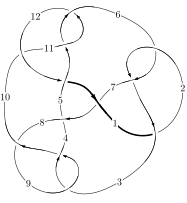
\includegraphics[width=112pt]{../../../GIT/diagram.site/Diagrams/png/1362_12a_0561.png}\\
\ \ \ A knot diagram\footnotemark}&
\allowdisplaybreaks
\textbf{Linearized knot diagam} \\
\cline{2-2}
 &
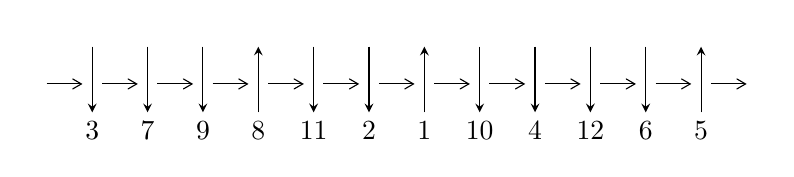
\begin{tikzpicture}[x=20pt, y=17pt]
	% nodes
	\node (C0) at (0, 0) {};
	\node (C1) at (1, 0) {};
	\node (C1U) at (1, +1) {};
	\node (C1D) at (1, -1) {3};

	\node (C2) at (2, 0) {};
	\node (C2U) at (2, +1) {};
	\node (C2D) at (2, -1) {7};

	\node (C3) at (3, 0) {};
	\node (C3U) at (3, +1) {};
	\node (C3D) at (3, -1) {9};

	\node (C4) at (4, 0) {};
	\node (C4U) at (4, +1) {};
	\node (C4D) at (4, -1) {8};

	\node (C5) at (5, 0) {};
	\node (C5U) at (5, +1) {};
	\node (C5D) at (5, -1) {11};

	\node (C6) at (6, 0) {};
	\node (C6U) at (6, +1) {};
	\node (C6D) at (6, -1) {2};

	\node (C7) at (7, 0) {};
	\node (C7U) at (7, +1) {};
	\node (C7D) at (7, -1) {1};

	\node (C8) at (8, 0) {};
	\node (C8U) at (8, +1) {};
	\node (C8D) at (8, -1) {10};

	\node (C9) at (9, 0) {};
	\node (C9U) at (9, +1) {};
	\node (C9D) at (9, -1) {4};

	\node (C10) at (10, 0) {};
	\node (C10U) at (10, +1) {};
	\node (C10D) at (10, -1) {12};

	\node (C11) at (11, 0) {};
	\node (C11U) at (11, +1) {};
	\node (C11D) at (11, -1) {6};

	\node (C12) at (12, 0) {};
	\node (C12U) at (12, +1) {};
	\node (C12D) at (12, -1) {5};
	\node (C13) at (13, 0) {};

	% arrows
	\draw[->,>={angle 60}]
	(C0) edge (C1) (C1) edge (C2) (C2) edge (C3) (C3) edge (C4) (C4) edge (C5) (C5) edge (C6) (C6) edge (C7) (C7) edge (C8) (C8) edge (C9) (C9) edge (C10) (C10) edge (C11) (C11) edge (C12) (C12) edge (C13) ;	\draw[->,>=stealth]
	(C1U) edge (C1D) (C2U) edge (C2D) (C3U) edge (C3D) (C4D) edge (C4U) (C5U) edge (C5D) (C6U) edge (C6D) (C7D) edge (C7U) (C8U) edge (C8D) (C9U) edge (C9D) (C10U) edge (C10D) (C11U) edge (C11D) (C12D) edge (C12U) ;
	\end{tikzpicture} \\
\hhline{~~} \\& 
\textbf{Solving Sequence} \\ \cline{2-2} 
 &
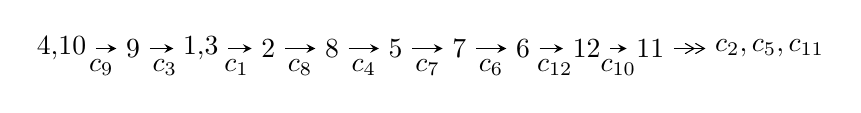
\begin{tikzpicture}[x=23pt, y=7pt]
	% node
	\node (A0) at (-1/8, 0) {4,10};
	\node (A1) at (1, 0) {9};
	\node (A2) at (33/16, 0) {1,3};
	\node (A3) at (25/8, 0) {2};
	\node (A4) at (33/8, 0) {8};
	\node (A5) at (41/8, 0) {5};
	\node (A6) at (49/8, 0) {7};
	\node (A7) at (57/8, 0) {6};
	\node (A8) at (65/8, 0) {12};
	\node (A9) at (73/8, 0) {11};
	\node (C1) at (1/2, -1) {$c_{9}$};
	\node (C2) at (3/2, -1) {$c_{3}$};
	\node (C3) at (21/8, -1) {$c_{1}$};
	\node (C4) at (29/8, -1) {$c_{8}$};
	\node (C5) at (37/8, -1) {$c_{4}$};
	\node (C6) at (45/8, -1) {$c_{7}$};
	\node (C7) at (53/8, -1) {$c_{6}$};
	\node (C8) at (61/8, -1) {$c_{12}$};
	\node (C9) at (69/8, -1) {$c_{10}$};
	\node (A10) at (11, 0) {$c_{2},c_{5},c_{11}$};

	% edge
	\draw[->,>=stealth]	
	(A0) edge (A1) (A1) edge (A2) (A2) edge (A3) (A3) edge (A4) (A4) edge (A5) (A5) edge (A6) (A6) edge (A7) (A7) edge (A8) (A8) edge (A9) ;
	\draw[->>,>={angle 60}]	
	(A9) edge (A10);
\end{tikzpicture} \\ 

\end{tabular} \\

\footnotetext{
The image of knot diagram is generated by the software ``\textbf{Draw programme}" developed by Andrew Bartholomew(\url{http://www.layer8.co.uk/maths/draw/index.htm\#Running-draw}), where we modified some parts for our purpose(\url{https://github.com/CATsTAILs/LinksPainter}).
}\phantom \\ \newline 
\centering \textbf{Ideals for irreducible components\footnotemark of $X_{\text{par}}$} 
 
\begin{align*}
I^u_{1}&=\langle 
- u^5+u^3- u^2+b- u,\;- u^5+2 u^3- u^2+a- u+1,\;u^7-2 u^5+u^4+2 u^3- u^2+u+1\rangle \\
I^u_{2}&=\langle 
u^8-2 u^6+2 u^4+b,\;u^{23}- u^{22}+\cdots+2 a+3,\;u^{24}+u^{23}+\cdots+2 u+1\rangle \\
I^u_{3}&=\langle 
u^{23}-5 u^{21}+\cdots+2 b- u,\;2 u^{23}+u^{22}+\cdots+2 a+1,\;u^{24}+u^{23}+\cdots+2 u+1\rangle \\
I^u_{4}&=\langle 
-9 u^{23}+30 u^{22}+\cdots+4 b+26,\;u^{23}-10 u^{22}+\cdots+8 a-34,\;u^{24}-4 u^{23}+\cdots-12 u+4\rangle \\
I^u_{5}&=\langle 
- u^2+b,\;- u^3- u^2+a+1,\;u^4- u^2+1\rangle \\
I^u_{6}&=\langle 
3 u^{23} a+2 u^{23}+\cdots+2 a+8,\;8 u^{23} a+2 u^{22} a+\cdots+6 a+4,\;u^{24}+u^{23}+\cdots+2 u^3+1\rangle \\
I^u_{7}&=\langle 
- u^2+b,\;u^3- u^2+a- u+1,\;u^4- u^2+1\rangle \\
I^u_{8}&=\langle 
u^2+b-1,\;- u^3+a-1,\;u^4- u^2+1\rangle \\
I^u_{9}&=\langle 
u^2+b-1,\;u^3+a- u-1,\;u^4- u^2+1\rangle \\
I^u_{10}&=\langle 
b+1,\;a,\;u-1\rangle \\
\\
\end{align*}
\raggedright * 10 irreducible components of $\dim_{\mathbb{C}}=0$, with total 144 representations.\\
\footnotetext{All coefficients of polynomials are rational numbers. But the coefficients are sometimes approximated in decimal forms when there is not enough margin.}
\newpage
\renewcommand{\arraystretch}{1}
\centering \section*{I. $I^u_{1}= \langle - u^5+u^3- u^2+b- u,\;- u^5+2 u^3- u^2+a- u+1,\;u^7-2 u^5+u^4+2 u^3- u^2+u+1 \rangle$}
\flushleft \textbf{(i) Arc colorings}\\
\begin{tabular}{m{7pt} m{180pt} m{7pt} m{180pt} }
\flushright $a_{4}=$&$\begin{pmatrix}0\\u\end{pmatrix}$ \\
\flushright $a_{10}=$&$\begin{pmatrix}1\\0\end{pmatrix}$ \\
\flushright $a_{9}=$&$\begin{pmatrix}1\\- u^2\end{pmatrix}$ \\
\flushright $a_{1}=$&$\begin{pmatrix}u^5-2 u^3+u^2+u-1\\u^5- u^3+u^2+u\end{pmatrix}$ \\
\flushright $a_{3}=$&$\begin{pmatrix}u\\- u^3+u\end{pmatrix}$ \\
\flushright $a_{2}=$&$\begin{pmatrix}u^5- u^3+u^2+u-1\\u^2+u\end{pmatrix}$ \\
\flushright $a_{8}=$&$\begin{pmatrix}- u^2+1\\- u^2\end{pmatrix}$ \\
\flushright $a_{5}=$&$\begin{pmatrix}u^5-2 u^3+u\\u^5- u^3+u\end{pmatrix}$ \\
\flushright $a_{7}=$&$\begin{pmatrix}u^6- u^4+u^3+u^2+1\\u^2+u\end{pmatrix}$ \\
\flushright $a_{6}=$&$\begin{pmatrix}u+1\\- u^3+u\end{pmatrix}$ \\
\flushright $a_{12}=$&$\begin{pmatrix}- u^6+u^4- u^3- u^2-1\\- u^2\end{pmatrix}$ \\
\flushright $a_{11}=$&$\begin{pmatrix}u^6- u^4+u^3- u+1\\u^4\end{pmatrix}$\\&\end{tabular}
\flushleft \textbf{(ii) Obstruction class $= -1$}\\~\\
\flushleft \textbf{(iii) Cusp Shapes $= 6 u^4-6 u^2+6 u-6$}\\~\\
\newpage\renewcommand{\arraystretch}{1}
\flushleft \textbf{(iv) u-Polynomials at the component}\newline \\
\begin{tabular}{m{50pt}|m{274pt}}
Crossings & \hspace{64pt}u-Polynomials at each crossing \\
\hline $$\begin{aligned}c_{1},c_{8},c_{10}\end{aligned}$$&$\begin{aligned}
&u^7+4 u^6+8 u^5+7 u^4+2 u^3- u^2+3 u+1
\end{aligned}$\\
\hline $$\begin{aligned}c_{2},c_{3},c_{5}\\c_{6},c_{9},c_{11}\end{aligned}$$&$\begin{aligned}
&u^7-2 u^5+u^4+2 u^3- u^2+u+1
\end{aligned}$\\
\hline $$\begin{aligned}c_{4},c_{7},c_{12}\end{aligned}$$&$\begin{aligned}
&u^7-3 u^6+8 u^5-10 u^4+12 u^3-6 u^2+3 u+3
\end{aligned}$\\
\hline
\end{tabular}\\~\\
\newpage\renewcommand{\arraystretch}{1}
\flushleft \textbf{(v) Riley Polynomials at the component}\newline \\
\begin{tabular}{m{50pt}|m{274pt}}
Crossings & \hspace{64pt}Riley Polynomials at each crossing \\
\hline $$\begin{aligned}c_{1},c_{8},c_{10}\end{aligned}$$&$\begin{aligned}
&y^7+12 y^5-3 y^4+58 y^3-3 y^2+11 y-1
\end{aligned}$\\
\hline $$\begin{aligned}c_{2},c_{3},c_{5}\\c_{6},c_{9},c_{11}\end{aligned}$$&$\begin{aligned}
&y^7-4 y^6+8 y^5-7 y^4+2 y^3+y^2+3 y-1
\end{aligned}$\\
\hline $$\begin{aligned}c_{4},c_{7},c_{12}\end{aligned}$$&$\begin{aligned}
&y^7+7 y^6+28 y^5+62 y^4+90 y^3+96 y^2+45 y-9
\end{aligned}$\\
\hline
\end{tabular}\\~\\
\newpage\flushleft \textbf{(vi) Complex Volumes and Cusp Shapes}
$$\begin{array}{c|c|c}  
\text{Solutions to }I^u_{1}& \I (\text{vol} + \sqrt{-1}CS) & \text{Cusp shape}\\
 \hline 
\begin{aligned}
u &= \phantom{-}0.323321 + 0.751928 I \\
a &= \phantom{-}0.22091 + 1.45384 I \\
b &= \phantom{-}0.70630 + 1.26451 I\end{aligned}
 & \phantom{-}1.50830 + 2.81502 I & -1.43908 - 1.09480 I \\ \hline\begin{aligned}
u &= \phantom{-}0.323321 - 0.751928 I \\
a &= \phantom{-}0.22091 - 1.45384 I \\
b &= \phantom{-}0.70630 - 1.26451 I\end{aligned}
 & \phantom{-}1.50830 - 2.81502 I & -1.43908 + 1.09480 I \\ \hline\begin{aligned}
u &= -1.209760 + 0.381906 I \\
a &= \phantom{-}1.45272 - 0.50136 I \\
b &= \phantom{-}1.21155 + 1.11972 I\end{aligned}
 & -10.84690 + 7.59135 I & -15.8701 - 6.7751 I \\ \hline\begin{aligned}
u &= -1.209760 - 0.381906 I \\
a &= \phantom{-}1.45272 + 0.50136 I \\
b &= \phantom{-}1.21155 - 1.11972 I\end{aligned}
 & -10.84690 - 7.59135 I & -15.8701 + 6.7751 I \\ \hline\begin{aligned}
u &= \phantom{-}1.159800 + 0.592772 I \\
a &= -2.18871 + 0.23437 I \\
b &= -0.85122 + 2.41814 I\end{aligned}
 & -5.8285 - 18.2895 I & -10.4221 + 11.7034 I \\ \hline\begin{aligned}
u &= \phantom{-}1.159800 - 0.592772 I \\
a &= -2.18871 - 0.23437 I \\
b &= -0.85122 - 2.41814 I\end{aligned}
 & -5.8285 + 18.2895 I & -10.4221 - 11.7034 I \\ \hline\begin{aligned}
u &= -0.546712\phantom{ +0.000000I} \\
a &= -0.969843\phantom{ +0.000000I} \\
b &= -0.133251\phantom{ +0.000000I}\end{aligned}
 & -0.919438\phantom{ +0.000000I} & -10.5380\phantom{ +0.000000I}\\
 \hline 
 \end{array}$$\newpage\newpage\renewcommand{\arraystretch}{1}
\centering \section*{II. $I^u_{2}= \langle u^8-2 u^6+2 u^4+b,\;u^{23}- u^{22}+\cdots+2 a+3,\;u^{24}+u^{23}+\cdots+2 u+1 \rangle$}
\flushleft \textbf{(i) Arc colorings}\\
\begin{tabular}{m{7pt} m{180pt} m{7pt} m{180pt} }
\flushright $a_{4}=$&$\begin{pmatrix}0\\u\end{pmatrix}$ \\
\flushright $a_{10}=$&$\begin{pmatrix}1\\0\end{pmatrix}$ \\
\flushright $a_{9}=$&$\begin{pmatrix}1\\- u^2\end{pmatrix}$ \\
\flushright $a_{1}=$&$\begin{pmatrix}-\frac{1}{2} u^{23}+\frac{1}{2} u^{22}+\cdots- u-\frac{3}{2}\\- u^8+2 u^6-2 u^4\end{pmatrix}$ \\
\flushright $a_{3}=$&$\begin{pmatrix}u\\- u^3+u\end{pmatrix}$ \\
\flushright $a_{2}=$&$\begin{pmatrix}- u^{23}+u^{22}+\cdots-2 u-2\\\frac{1}{2} u^{22}-\frac{5}{2} u^{20}+\cdots+\frac{1}{2} u+\frac{1}{2}\end{pmatrix}$ \\
\flushright $a_{8}=$&$\begin{pmatrix}- u^2+1\\- u^2\end{pmatrix}$ \\
\flushright $a_{5}=$&$\begin{pmatrix}u^5-2 u^3+u\\u^5- u^3+u\end{pmatrix}$ \\
\flushright $a_{7}=$&$\begin{pmatrix}\frac{3}{2} u^{23}-\frac{21}{2} u^{21}+\cdots+\frac{5}{2} u+3\\\frac{1}{2} u^{22}-\frac{5}{2} u^{20}+\cdots+\frac{1}{2} u+\frac{1}{2}\end{pmatrix}$ \\
\flushright $a_{6}=$&$\begin{pmatrix}\frac{1}{2} u^{23}+\frac{1}{2} u^{22}+\cdots-\frac{3}{2} u^2+\frac{1}{2}\\- u^3+u\end{pmatrix}$ \\
\flushright $a_{12}=$&$\begin{pmatrix}-\frac{1}{2} u^{23}+\frac{1}{2} u^{22}+\cdots- u-\frac{3}{2}\\- u^2\end{pmatrix}$ \\
\flushright $a_{11}=$&$\begin{pmatrix}\frac{1}{2} u^{23}-\frac{7}{2} u^{21}+\cdots+\frac{3}{2} u+2\\u^4\end{pmatrix}$\\&\end{tabular}
\flushleft \textbf{(ii) Obstruction class $= -1$}\\~\\
\flushleft \textbf{(iii) Cusp Shapes $= -2 u^{23}+16 u^{21}+2 u^{20}-60 u^{19}-14 u^{18}+132 u^{17}+50 u^{16}-176 u^{15}-108 u^{14}+124 u^{13}+152 u^{12}-4 u^{11}-134 u^{10}-68 u^9+66 u^8+50 u^7-8 u^6-16 u^5-2 u^4+12 u^3+2 u^2-8 u-12$}\\~\\
\newpage\renewcommand{\arraystretch}{1}
\flushleft \textbf{(iv) u-Polynomials at the component}\newline \\
\begin{tabular}{m{50pt}|m{274pt}}
Crossings & \hspace{64pt}u-Polynomials at each crossing \\
\hline $$\begin{aligned}c_{1}\end{aligned}$$&$\begin{aligned}
&u^{24}+10 u^{23}+\cdots+24 u+16
\end{aligned}$\\
\hline $$\begin{aligned}c_{2},c_{6}\end{aligned}$$&$\begin{aligned}
&u^{24}-4 u^{23}+\cdots-12 u+4
\end{aligned}$\\
\hline $$\begin{aligned}c_{3},c_{5},c_{9}\\c_{11}\end{aligned}$$&$\begin{aligned}
&u^{24}+u^{23}+\cdots+2 u+1
\end{aligned}$\\
\hline $$\begin{aligned}c_{4},c_{12}\end{aligned}$$&$\begin{aligned}
&u^{24}+3 u^{23}+\cdots+8 u+3
\end{aligned}$\\
\hline $$\begin{aligned}c_{7}\end{aligned}$$&$\begin{aligned}
&u^{24}-12 u^{23}+\cdots-1436 u+276
\end{aligned}$\\
\hline $$\begin{aligned}c_{8},c_{10}\end{aligned}$$&$\begin{aligned}
&u^{24}+13 u^{23}+\cdots+4 u+1
\end{aligned}$\\
\hline
\end{tabular}\\~\\
\newpage\renewcommand{\arraystretch}{1}
\flushleft \textbf{(v) Riley Polynomials at the component}\newline \\
\begin{tabular}{m{50pt}|m{274pt}}
Crossings & \hspace{64pt}Riley Polynomials at each crossing \\
\hline $$\begin{aligned}c_{1}\end{aligned}$$&$\begin{aligned}
&y^{24}+6 y^{23}+\cdots+1248 y+256
\end{aligned}$\\
\hline $$\begin{aligned}c_{2},c_{6}\end{aligned}$$&$\begin{aligned}
&y^{24}-10 y^{23}+\cdots-24 y+16
\end{aligned}$\\
\hline $$\begin{aligned}c_{3},c_{5},c_{9}\\c_{11}\end{aligned}$$&$\begin{aligned}
&y^{24}-13 y^{23}+\cdots-4 y+1
\end{aligned}$\\
\hline $$\begin{aligned}c_{4},c_{12}\end{aligned}$$&$\begin{aligned}
&y^{24}+15 y^{23}+\cdots-46 y+9
\end{aligned}$\\
\hline $$\begin{aligned}c_{7}\end{aligned}$$&$\begin{aligned}
&y^{24}-2 y^{23}+\cdots+176264 y+76176
\end{aligned}$\\
\hline $$\begin{aligned}c_{8},c_{10}\end{aligned}$$&$\begin{aligned}
&y^{24}- y^{23}+\cdots+4 y+1
\end{aligned}$\\
\hline
\end{tabular}\\~\\
\newpage\flushleft \textbf{(vi) Complex Volumes and Cusp Shapes}
$$\begin{array}{c|c|c}  
\text{Solutions to }I^u_{2}& \I (\text{vol} + \sqrt{-1}CS) & \text{Cusp shape}\\
 \hline 
\begin{aligned}
u &= \phantom{-}0.872385 + 0.264900 I \\
a &= -0.323474 + 1.214120 I \\
b &= -0.415052 - 0.487887 I\end{aligned}
 & -1.33365 - 4.85950 I & -12.45920 + 5.77046 I \\ \hline\begin{aligned}
u &= \phantom{-}0.872385 - 0.264900 I \\
a &= -0.323474 - 1.214120 I \\
b &= -0.415052 + 0.487887 I\end{aligned}
 & -1.33365 + 4.85950 I & -12.45920 - 5.77046 I \\ \hline\begin{aligned}
u &= -0.315716 + 0.809370 I \\
a &= \phantom{-}0.33853 - 2.31494 I \\
b &= \phantom{-}0.75319 - 1.86800 I\end{aligned}
 & -0.85756 - 7.78163 I & -4.85194 + 4.83472 I \\ \hline\begin{aligned}
u &= -0.315716 - 0.809370 I \\
a &= \phantom{-}0.33853 + 2.31494 I \\
b &= \phantom{-}0.75319 + 1.86800 I\end{aligned}
 & -0.85756 + 7.78163 I & -4.85194 - 4.83472 I \\ \hline\begin{aligned}
u &= \phantom{-}1.085000 + 0.487361 I \\
a &= \phantom{-}0.851652 - 0.459018 I \\
b &= -0.280563 + 0.198174 I\end{aligned}
 & -1.84490 - 4.33375 I & -10.12719 + 4.87141 I \\ \hline\begin{aligned}
u &= \phantom{-}1.085000 - 0.487361 I \\
a &= \phantom{-}0.851652 + 0.459018 I \\
b &= -0.280563 - 0.198174 I\end{aligned}
 & -1.84490 + 4.33375 I & -10.12719 - 4.87141 I \\ \hline\begin{aligned}
u &= -0.756777 + 0.219796 I \\
a &= -0.947046 - 0.628257 I \\
b &= -0.293717 + 0.337217 I\end{aligned}
 & -0.610616 + 0.203500 I & -9.13505 + 0.22341 I \\ \hline\begin{aligned}
u &= -0.756777 - 0.219796 I \\
a &= -0.947046 + 0.628257 I \\
b &= -0.293717 - 0.337217 I\end{aligned}
 & -0.610616 - 0.203500 I & -9.13505 - 0.22341 I \\ \hline\begin{aligned}
u &= \phantom{-}1.170110 + 0.334879 I \\
a &= \phantom{-}1.225630 + 0.246296 I \\
b &= \phantom{-}0.357167 - 1.279390 I\end{aligned}
 & -6.89501 - 3.48528 I & -12.35004 + 3.84640 I \\ \hline\begin{aligned}
u &= \phantom{-}1.170110 - 0.334879 I \\
a &= \phantom{-}1.225630 - 0.246296 I \\
b &= \phantom{-}0.357167 + 1.279390 I\end{aligned}
 & -6.89501 + 3.48528 I & -12.35004 - 3.84640 I\\
 \hline 
 \end{array}$$\newpage$$\begin{array}{c|c|c}  
\text{Solutions to }I^u_{2}& \I (\text{vol} + \sqrt{-1}CS) & \text{Cusp shape}\\
 \hline 
\begin{aligned}
u &= -1.100620 + 0.522247 I \\
a &= \phantom{-}0.139238 + 0.659699 I \\
b &= -0.444574 - 0.623609 I\end{aligned}
 & -1.15502 + 9.82269 I & -8.18318 - 9.91604 I \\ \hline\begin{aligned}
u &= -1.100620 - 0.522247 I \\
a &= \phantom{-}0.139238 - 0.659699 I \\
b &= -0.444574 + 0.623609 I\end{aligned}
 & -1.15502 - 9.82269 I & -8.18318 + 9.91604 I \\ \hline\begin{aligned}
u &= -0.192309 + 0.742887 I \\
a &= -1.22926 - 1.35826 I \\
b &= -0.334849 - 1.104320 I\end{aligned}
 & -2.86629 - 0.02006 I & -7.67881 - 0.81568 I \\ \hline\begin{aligned}
u &= -0.192309 - 0.742887 I \\
a &= -1.22926 + 1.35826 I \\
b &= -0.334849 + 1.104320 I\end{aligned}
 & -2.86629 + 0.02006 I & -7.67881 + 0.81568 I \\ \hline\begin{aligned}
u &= -0.516542 + 0.554919 I \\
a &= -0.458840 + 0.974457 I \\
b &= \phantom{-}0.630180 + 0.307536 I\end{aligned}
 & \phantom{-}1.74238 + 4.07387 I & -2.10471 - 4.89426 I \\ \hline\begin{aligned}
u &= -0.516542 - 0.554919 I \\
a &= -0.458840 - 0.974457 I \\
b &= \phantom{-}0.630180 - 0.307536 I\end{aligned}
 & \phantom{-}1.74238 - 4.07387 I & -2.10471 + 4.89426 I \\ \hline\begin{aligned}
u &= -1.210320 + 0.293868 I \\
a &= \phantom{-}1.282240 + 0.074124 I \\
b &= \phantom{-}0.16762 + 2.00067 I\end{aligned}
 & -10.16720 - 1.16183 I & -15.8009 + 0.1079 I \\ \hline\begin{aligned}
u &= -1.210320 - 0.293868 I \\
a &= \phantom{-}1.282240 - 0.074124 I \\
b &= \phantom{-}0.16762 - 2.00067 I\end{aligned}
 & -10.16720 + 1.16183 I & -15.8009 - 0.1079 I \\ \hline\begin{aligned}
u &= \phantom{-}0.439637 + 0.612670 I \\
a &= \phantom{-}0.066881 - 0.351296 I \\
b &= \phantom{-}0.791483 + 0.085996 I\end{aligned}
 & \phantom{-}2.85828 + 0.77209 I & \phantom{-}0.169658 - 0.914191 I \\ \hline\begin{aligned}
u &= \phantom{-}0.439637 - 0.612670 I \\
a &= \phantom{-}0.066881 + 0.351296 I \\
b &= \phantom{-}0.791483 - 0.085996 I\end{aligned}
 & \phantom{-}2.85828 - 0.77209 I & \phantom{-}0.169658 + 0.914191 I\\
 \hline 
 \end{array}$$\newpage$$\begin{array}{c|c|c}  
\text{Solutions to }I^u_{2}& \I (\text{vol} + \sqrt{-1}CS) & \text{Cusp shape}\\
 \hline 
\begin{aligned}
u &= -1.148140 + 0.576039 I \\
a &= -1.58681 + 0.02147 I \\
b &= -0.67603 - 1.92774 I\end{aligned}
 & -3.32912 + 12.94620 I & -7.81680 - 8.29853 I \\ \hline\begin{aligned}
u &= -1.148140 - 0.576039 I \\
a &= -1.58681 - 0.02147 I \\
b &= -0.67603 + 1.92774 I\end{aligned}
 & -3.32912 - 12.94620 I & -7.81680 + 8.29853 I \\ \hline\begin{aligned}
u &= \phantom{-}1.173300 + 0.546469 I \\
a &= -0.858733 + 0.794056 I \\
b &= \phantom{-}0.24514 + 1.86122 I\end{aligned}
 & -8.44001 - 9.78226 I & -13.6619 + 6.4188 I \\ \hline\begin{aligned}
u &= \phantom{-}1.173300 - 0.546469 I \\
a &= -0.858733 - 0.794056 I \\
b &= \phantom{-}0.24514 - 1.86122 I\end{aligned}
 & -8.44001 + 9.78226 I & -13.6619 - 6.4188 I\\
 \hline 
 \end{array}$$\newpage\newpage\renewcommand{\arraystretch}{1}
\centering \section*{III. $I^u_{3}= \langle u^{23}-5 u^{21}+\cdots+2 b- u,\;2 u^{23}+u^{22}+\cdots+2 a+1,\;u^{24}+u^{23}+\cdots+2 u+1 \rangle$}
\flushleft \textbf{(i) Arc colorings}\\
\begin{tabular}{m{7pt} m{180pt} m{7pt} m{180pt} }
\flushright $a_{4}=$&$\begin{pmatrix}0\\u\end{pmatrix}$ \\
\flushright $a_{10}=$&$\begin{pmatrix}1\\0\end{pmatrix}$ \\
\flushright $a_{9}=$&$\begin{pmatrix}1\\- u^2\end{pmatrix}$ \\
\flushright $a_{1}=$&$\begin{pmatrix}- u^{23}-\frac{1}{2} u^{22}+\cdots+\frac{3}{2} u-\frac{1}{2}\\-\frac{1}{2} u^{23}+\frac{5}{2} u^{21}+\cdots-\frac{1}{2} u^2+\frac{1}{2} u\end{pmatrix}$ \\
\flushright $a_{3}=$&$\begin{pmatrix}u\\- u^3+u\end{pmatrix}$ \\
\flushright $a_{2}=$&$\begin{pmatrix}- u^{23}-\frac{1}{2} u^{22}+\cdots+\frac{3}{2} u-\frac{1}{2}\\-\frac{1}{2} u^{23}+\frac{5}{2} u^{21}+\cdots-\frac{1}{2} u^2+\frac{1}{2} u\end{pmatrix}$ \\
\flushright $a_{8}=$&$\begin{pmatrix}- u^2+1\\- u^2\end{pmatrix}$ \\
\flushright $a_{5}=$&$\begin{pmatrix}u^5-2 u^3+u\\u^5- u^3+u\end{pmatrix}$ \\
\flushright $a_{7}=$&$\begin{pmatrix}\frac{1}{2} u^{23}-\frac{1}{2} u^{22}+\cdots+u+\frac{3}{2}\\-\frac{1}{2} u^{22}+\frac{5}{2} u^{20}+\cdots-\frac{1}{2} u-\frac{1}{2}\end{pmatrix}$ \\
\flushright $a_{6}=$&$\begin{pmatrix}-\frac{1}{2} u^{22}+\frac{5}{2} u^{20}+\cdots-\frac{1}{2} u+\frac{1}{2}\\-\frac{1}{2} u^{23}+\frac{7}{2} u^{21}+\cdots-\frac{3}{2} u-1\end{pmatrix}$ \\
\flushright $a_{12}=$&$\begin{pmatrix}-\frac{3}{2} u^{23}-\frac{1}{2} u^{22}+\cdots+u-\frac{1}{2}\\-\frac{1}{2} u^{23}+\frac{5}{2} u^{21}+\cdots-\frac{1}{2} u^2+\frac{1}{2} u\end{pmatrix}$ \\
\flushright $a_{11}=$&$\begin{pmatrix}\frac{5}{2} u^{23}+\frac{1}{2} u^{22}+\cdots+u+\frac{1}{2}\\\frac{1}{2} u^{23}+\frac{1}{2} u^{22}+\cdots- u-\frac{3}{2}\end{pmatrix}$\\&\end{tabular}
\flushleft \textbf{(ii) Obstruction class $= -1$}\\~\\
\flushleft \textbf{(iii) Cusp Shapes $= -2 u^{23}+16 u^{21}+2 u^{20}-60 u^{19}-14 u^{18}+132 u^{17}+50 u^{16}-176 u^{15}-108 u^{14}+124 u^{13}+152 u^{12}-4 u^{11}-134 u^{10}-68 u^9+66 u^8+50 u^7-8 u^6-16 u^5-2 u^4+12 u^3+2 u^2-8 u-12$}\\~\\
\newpage\renewcommand{\arraystretch}{1}
\flushleft \textbf{(iv) u-Polynomials at the component}\newline \\
\begin{tabular}{m{50pt}|m{274pt}}
Crossings & \hspace{64pt}u-Polynomials at each crossing \\
\hline $$\begin{aligned}c_{1},c_{8}\end{aligned}$$&$\begin{aligned}
&u^{24}+13 u^{23}+\cdots+4 u+1
\end{aligned}$\\
\hline $$\begin{aligned}c_{2},c_{3},c_{6}\\c_{9}\end{aligned}$$&$\begin{aligned}
&u^{24}+u^{23}+\cdots+2 u+1
\end{aligned}$\\
\hline $$\begin{aligned}c_{4},c_{7}\end{aligned}$$&$\begin{aligned}
&u^{24}+3 u^{23}+\cdots+8 u+3
\end{aligned}$\\
\hline $$\begin{aligned}c_{5},c_{11}\end{aligned}$$&$\begin{aligned}
&u^{24}-4 u^{23}+\cdots-12 u+4
\end{aligned}$\\
\hline $$\begin{aligned}c_{10}\end{aligned}$$&$\begin{aligned}
&u^{24}+10 u^{23}+\cdots+24 u+16
\end{aligned}$\\
\hline $$\begin{aligned}c_{12}\end{aligned}$$&$\begin{aligned}
&u^{24}-12 u^{23}+\cdots-1436 u+276
\end{aligned}$\\
\hline
\end{tabular}\\~\\
\newpage\renewcommand{\arraystretch}{1}
\flushleft \textbf{(v) Riley Polynomials at the component}\newline \\
\begin{tabular}{m{50pt}|m{274pt}}
Crossings & \hspace{64pt}Riley Polynomials at each crossing \\
\hline $$\begin{aligned}c_{1},c_{8}\end{aligned}$$&$\begin{aligned}
&y^{24}- y^{23}+\cdots+4 y+1
\end{aligned}$\\
\hline $$\begin{aligned}c_{2},c_{3},c_{6}\\c_{9}\end{aligned}$$&$\begin{aligned}
&y^{24}-13 y^{23}+\cdots-4 y+1
\end{aligned}$\\
\hline $$\begin{aligned}c_{4},c_{7}\end{aligned}$$&$\begin{aligned}
&y^{24}+15 y^{23}+\cdots-46 y+9
\end{aligned}$\\
\hline $$\begin{aligned}c_{5},c_{11}\end{aligned}$$&$\begin{aligned}
&y^{24}-10 y^{23}+\cdots-24 y+16
\end{aligned}$\\
\hline $$\begin{aligned}c_{10}\end{aligned}$$&$\begin{aligned}
&y^{24}+6 y^{23}+\cdots+1248 y+256
\end{aligned}$\\
\hline $$\begin{aligned}c_{12}\end{aligned}$$&$\begin{aligned}
&y^{24}-2 y^{23}+\cdots+176264 y+76176
\end{aligned}$\\
\hline
\end{tabular}\\~\\
\newpage\flushleft \textbf{(vi) Complex Volumes and Cusp Shapes}
$$\begin{array}{c|c|c}  
\text{Solutions to }I^u_{3}& \I (\text{vol} + \sqrt{-1}CS) & \text{Cusp shape}\\
 \hline 
\begin{aligned}
u &= \phantom{-}0.872385 + 0.264900 I \\
a &= \phantom{-}0.93475 - 1.40984 I \\
b &= -1.23505 - 1.13274 I\end{aligned}
 & -1.33365 - 4.85950 I & -12.45920 + 5.77046 I \\ \hline\begin{aligned}
u &= \phantom{-}0.872385 - 0.264900 I \\
a &= \phantom{-}0.93475 + 1.40984 I \\
b &= -1.23505 + 1.13274 I\end{aligned}
 & -1.33365 + 4.85950 I & -12.45920 - 5.77046 I \\ \hline\begin{aligned}
u &= -0.315716 + 0.809370 I \\
a &= -0.14253 + 1.46556 I \\
b &= -0.65497 + 1.39733 I\end{aligned}
 & -0.85756 - 7.78163 I & -4.85194 + 4.83472 I \\ \hline\begin{aligned}
u &= -0.315716 - 0.809370 I \\
a &= -0.14253 - 1.46556 I \\
b &= -0.65497 - 1.39733 I\end{aligned}
 & -0.85756 + 7.78163 I & -4.85194 - 4.83472 I \\ \hline\begin{aligned}
u &= \phantom{-}1.085000 + 0.487361 I \\
a &= -2.54924 - 0.76910 I \\
b &= -2.05211 + 2.16225 I\end{aligned}
 & -1.84490 - 4.33375 I & -10.12719 + 4.87141 I \\ \hline\begin{aligned}
u &= \phantom{-}1.085000 - 0.487361 I \\
a &= -2.54924 + 0.76910 I \\
b &= -2.05211 - 2.16225 I\end{aligned}
 & -1.84490 + 4.33375 I & -10.12719 - 4.87141 I \\ \hline\begin{aligned}
u &= -0.756777 + 0.219796 I \\
a &= -1.34088 - 0.49415 I \\
b &= \phantom{-}0.283448 - 0.900890 I\end{aligned}
 & -0.610616 + 0.203500 I & -9.13505 + 0.22341 I \\ \hline\begin{aligned}
u &= -0.756777 - 0.219796 I \\
a &= -1.34088 + 0.49415 I \\
b &= \phantom{-}0.283448 + 0.900890 I\end{aligned}
 & -0.610616 - 0.203500 I & -9.13505 - 0.22341 I \\ \hline\begin{aligned}
u &= \phantom{-}1.170110 + 0.334879 I \\
a &= -1.27442 - 0.69688 I \\
b &= -1.38871 + 0.84297 I\end{aligned}
 & -6.89501 - 3.48528 I & -12.35004 + 3.84640 I \\ \hline\begin{aligned}
u &= \phantom{-}1.170110 - 0.334879 I \\
a &= -1.27442 + 0.69688 I \\
b &= -1.38871 - 0.84297 I\end{aligned}
 & -6.89501 + 3.48528 I & -12.35004 - 3.84640 I\\
 \hline 
 \end{array}$$\newpage$$\begin{array}{c|c|c}  
\text{Solutions to }I^u_{3}& \I (\text{vol} + \sqrt{-1}CS) & \text{Cusp shape}\\
 \hline 
\begin{aligned}
u &= -1.100620 + 0.522247 I \\
a &= \phantom{-}2.57917 - 0.35492 I \\
b &= \phantom{-}1.66695 + 2.42094 I\end{aligned}
 & -1.15502 + 9.82269 I & -8.18318 - 9.91604 I \\ \hline\begin{aligned}
u &= -1.100620 - 0.522247 I \\
a &= \phantom{-}2.57917 + 0.35492 I \\
b &= \phantom{-}1.66695 - 2.42094 I\end{aligned}
 & -1.15502 - 9.82269 I & -8.18318 + 9.91604 I \\ \hline\begin{aligned}
u &= -0.192309 + 0.742887 I \\
a &= -0.145590 + 1.310270 I \\
b &= -0.402626 + 1.200440 I\end{aligned}
 & -2.86629 - 0.02006 I & -7.67881 - 0.81568 I \\ \hline\begin{aligned}
u &= -0.192309 - 0.742887 I \\
a &= -0.145590 - 1.310270 I \\
b &= -0.402626 - 1.200440 I\end{aligned}
 & -2.86629 + 0.02006 I & -7.67881 + 0.81568 I \\ \hline\begin{aligned}
u &= -0.516542 + 0.554919 I \\
a &= -0.97555 + 1.63616 I \\
b &= -1.43709 + 0.58926 I\end{aligned}
 & \phantom{-}1.74238 + 4.07387 I & -2.10471 - 4.89426 I \\ \hline\begin{aligned}
u &= -0.516542 - 0.554919 I \\
a &= -0.97555 - 1.63616 I \\
b &= -1.43709 - 0.58926 I\end{aligned}
 & \phantom{-}1.74238 - 4.07387 I & -2.10471 + 4.89426 I \\ \hline\begin{aligned}
u &= -1.210320 + 0.293868 I \\
a &= \phantom{-}1.131960 - 0.521366 I \\
b &= \phantom{-}1.152730 + 0.708697 I\end{aligned}
 & -10.16720 - 1.16183 I & -15.8009 + 0.1079 I \\ \hline\begin{aligned}
u &= -1.210320 - 0.293868 I \\
a &= \phantom{-}1.131960 + 0.521366 I \\
b &= \phantom{-}1.152730 - 0.708697 I\end{aligned}
 & -10.16720 + 1.16183 I & -15.8009 - 0.1079 I \\ \hline\begin{aligned}
u &= \phantom{-}0.439637 + 0.612670 I \\
a &= \phantom{-}0.61309 + 1.54085 I \\
b &= \phantom{-}1.11515 + 0.87846 I\end{aligned}
 & \phantom{-}2.85828 + 0.77209 I & \phantom{-}0.169658 - 0.914191 I \\ \hline\begin{aligned}
u &= \phantom{-}0.439637 - 0.612670 I \\
a &= \phantom{-}0.61309 - 1.54085 I \\
b &= \phantom{-}1.11515 - 0.87846 I\end{aligned}
 & \phantom{-}2.85828 - 0.77209 I & \phantom{-}0.169658 + 0.914191 I\\
 \hline 
 \end{array}$$\newpage$$\begin{array}{c|c|c}  
\text{Solutions to }I^u_{3}& \I (\text{vol} + \sqrt{-1}CS) & \text{Cusp shape}\\
 \hline 
\begin{aligned}
u &= -1.148140 + 0.576039 I \\
a &= \phantom{-}2.26759 + 0.13614 I \\
b &= \phantom{-}0.99891 + 2.42525 I\end{aligned}
 & -3.32912 + 12.94620 I & -7.81680 - 8.29853 I \\ \hline\begin{aligned}
u &= -1.148140 - 0.576039 I \\
a &= \phantom{-}2.26759 - 0.13614 I \\
b &= \phantom{-}0.99891 - 2.42525 I\end{aligned}
 & -3.32912 - 12.94620 I & -7.81680 + 8.29853 I \\ \hline\begin{aligned}
u &= \phantom{-}1.173300 + 0.546469 I \\
a &= -2.09835 - 0.02884 I \\
b &= -1.04662 + 2.14658 I\end{aligned}
 & -8.44001 - 9.78226 I & -13.6619 + 6.4188 I \\ \hline\begin{aligned}
u &= \phantom{-}1.173300 - 0.546469 I \\
a &= -2.09835 + 0.02884 I \\
b &= -1.04662 - 2.14658 I\end{aligned}
 & -8.44001 + 9.78226 I & -13.6619 - 6.4188 I\\
 \hline 
 \end{array}$$\newpage\newpage\renewcommand{\arraystretch}{1}
\centering \section*{IV. $I^u_{4}= \langle -9 u^{23}+30 u^{22}+\cdots+4 b+26,\;u^{23}-10 u^{22}+\cdots+8 a-34,\;u^{24}-4 u^{23}+\cdots-12 u+4 \rangle$}
\flushleft \textbf{(i) Arc colorings}\\
\begin{tabular}{m{7pt} m{180pt} m{7pt} m{180pt} }
\flushright $a_{4}=$&$\begin{pmatrix}0\\u\end{pmatrix}$ \\
\flushright $a_{10}=$&$\begin{pmatrix}1\\0\end{pmatrix}$ \\
\flushright $a_{9}=$&$\begin{pmatrix}1\\- u^2\end{pmatrix}$ \\
\flushright $a_{1}=$&$\begin{pmatrix}-\frac{1}{8} u^{23}+\frac{5}{4} u^{22}+\cdots-\frac{41}{8} u+\frac{17}{4}\\\frac{9}{4} u^{23}-\frac{15}{2} u^{22}+\cdots+\frac{81}{4} u-\frac{13}{2}\end{pmatrix}$ \\
\flushright $a_{3}=$&$\begin{pmatrix}u\\- u^3+u\end{pmatrix}$ \\
\flushright $a_{2}=$&$\begin{pmatrix}-0.625000 u^{23}+5.25000 u^{22}+\cdots-22.6250 u+15.2500\\-\frac{9}{4} u^{23}+\frac{15}{2} u^{22}+\cdots-\frac{93}{4} u+\frac{25}{2}\end{pmatrix}$ \\
\flushright $a_{8}=$&$\begin{pmatrix}- u^2+1\\- u^2\end{pmatrix}$ \\
\flushright $a_{5}=$&$\begin{pmatrix}u^5-2 u^3+u\\u^5- u^3+u\end{pmatrix}$ \\
\flushright $a_{7}=$&$\begin{pmatrix}\frac{9}{8} u^{23}-\frac{15}{4} u^{22}+\cdots+\frac{61}{8} u-\frac{7}{4}\\\frac{5}{4} u^{23}-\frac{7}{2} u^{22}+\cdots+\frac{25}{4} u-\frac{3}{2}\end{pmatrix}$ \\
\flushright $a_{6}=$&$\begin{pmatrix}\frac{49}{8} u^{23}-\frac{77}{4} u^{22}+\cdots+\frac{369}{8} u-\frac{57}{4}\\\frac{15}{4} u^{23}-\frac{21}{2} u^{22}+\cdots+\frac{83}{4} u-\frac{7}{2}\end{pmatrix}$ \\
\flushright $a_{12}=$&$\begin{pmatrix}\frac{3}{8} u^{23}-\frac{19}{4} u^{22}+\cdots+\frac{203}{8} u-\frac{67}{4}\\\frac{11}{4} u^{23}-\frac{21}{2} u^{22}+\cdots+\frac{131}{4} u-\frac{31}{2}\end{pmatrix}$ \\
\flushright $a_{11}=$&$\begin{pmatrix}-\frac{3}{8} u^{23}+\frac{5}{4} u^{22}+\cdots-\frac{55}{8} u+\frac{21}{4}\\-\frac{1}{4} u^{23}+\frac{1}{2} u^{22}+\cdots-\frac{9}{4} u+\frac{3}{2}\end{pmatrix}$\\&\end{tabular}
\flushleft \textbf{(ii) Obstruction class $= -1$}\\~\\
\flushleft \textbf{(iii) Cusp Shapes $= 4 u^{23}-20 u^{22}+12 u^{21}+78 u^{20}-128 u^{19}-88 u^{18}+340 u^{17}-98 u^{16}-440 u^{15}+420 u^{14}+232 u^{13}-598 u^{12}+174 u^{11}+404 u^{10}-406 u^9-36 u^8+290 u^7-156 u^6-76 u^5+126 u^4-26 u^3-58 u^2+56 u-18$}\\~\\
\newpage\renewcommand{\arraystretch}{1}
\flushleft \textbf{(iv) u-Polynomials at the component}\newline \\
\begin{tabular}{m{50pt}|m{274pt}}
Crossings & \hspace{64pt}u-Polynomials at each crossing \\
\hline $$\begin{aligned}c_{1},c_{10}\end{aligned}$$&$\begin{aligned}
&u^{24}+13 u^{23}+\cdots+4 u+1
\end{aligned}$\\
\hline $$\begin{aligned}c_{2},c_{5},c_{6}\\c_{11}\end{aligned}$$&$\begin{aligned}
&u^{24}+u^{23}+\cdots+2 u+1
\end{aligned}$\\
\hline $$\begin{aligned}c_{3},c_{9}\end{aligned}$$&$\begin{aligned}
&u^{24}-4 u^{23}+\cdots-12 u+4
\end{aligned}$\\
\hline $$\begin{aligned}c_{4}\end{aligned}$$&$\begin{aligned}
&u^{24}-12 u^{23}+\cdots-1436 u+276
\end{aligned}$\\
\hline $$\begin{aligned}c_{7},c_{12}\end{aligned}$$&$\begin{aligned}
&u^{24}+3 u^{23}+\cdots+8 u+3
\end{aligned}$\\
\hline $$\begin{aligned}c_{8}\end{aligned}$$&$\begin{aligned}
&u^{24}+10 u^{23}+\cdots+24 u+16
\end{aligned}$\\
\hline
\end{tabular}\\~\\
\newpage\renewcommand{\arraystretch}{1}
\flushleft \textbf{(v) Riley Polynomials at the component}\newline \\
\begin{tabular}{m{50pt}|m{274pt}}
Crossings & \hspace{64pt}Riley Polynomials at each crossing \\
\hline $$\begin{aligned}c_{1},c_{10}\end{aligned}$$&$\begin{aligned}
&y^{24}- y^{23}+\cdots+4 y+1
\end{aligned}$\\
\hline $$\begin{aligned}c_{2},c_{5},c_{6}\\c_{11}\end{aligned}$$&$\begin{aligned}
&y^{24}-13 y^{23}+\cdots-4 y+1
\end{aligned}$\\
\hline $$\begin{aligned}c_{3},c_{9}\end{aligned}$$&$\begin{aligned}
&y^{24}-10 y^{23}+\cdots-24 y+16
\end{aligned}$\\
\hline $$\begin{aligned}c_{4}\end{aligned}$$&$\begin{aligned}
&y^{24}-2 y^{23}+\cdots+176264 y+76176
\end{aligned}$\\
\hline $$\begin{aligned}c_{7},c_{12}\end{aligned}$$&$\begin{aligned}
&y^{24}+15 y^{23}+\cdots-46 y+9
\end{aligned}$\\
\hline $$\begin{aligned}c_{8}\end{aligned}$$&$\begin{aligned}
&y^{24}+6 y^{23}+\cdots+1248 y+256
\end{aligned}$\\
\hline
\end{tabular}\\~\\
\newpage\flushleft \textbf{(vi) Complex Volumes and Cusp Shapes}
$$\begin{array}{c|c|c}  
\text{Solutions to }I^u_{4}& \I (\text{vol} + \sqrt{-1}CS) & \text{Cusp shape}\\
 \hline 
\begin{aligned}
u &= \phantom{-}0.698657 + 0.763262 I \\
a &= \phantom{-}0.140948 + 0.781183 I \\
b &= -0.444574 + 0.623609 I\end{aligned}
 & -1.15502 - 9.82269 I & -8.18318 + 9.91604 I \\ \hline\begin{aligned}
u &= \phantom{-}0.698657 - 0.763262 I \\
a &= \phantom{-}0.140948 - 0.781183 I \\
b &= -0.444574 - 0.623609 I\end{aligned}
 & -1.15502 + 9.82269 I & -8.18318 - 9.91604 I \\ \hline\begin{aligned}
u &= \phantom{-}0.326549 + 0.852618 I \\
a &= -0.25129 - 2.21854 I \\
b &= -0.67603 - 1.92774 I\end{aligned}
 & -3.32912 + 12.94620 I & -7.81680 - 8.29853 I \\ \hline\begin{aligned}
u &= \phantom{-}0.326549 - 0.852618 I \\
a &= -0.25129 + 2.21854 I \\
b &= -0.67603 + 1.92774 I\end{aligned}
 & -3.32912 - 12.94620 I & -7.81680 + 8.29853 I \\ \hline\begin{aligned}
u &= -0.926567 + 0.601992 I \\
a &= -0.021753 + 1.036510 I \\
b &= -0.415052 + 0.487887 I\end{aligned}
 & -1.33365 + 4.85950 I & -12.45920 - 5.77046 I \\ \hline\begin{aligned}
u &= -0.926567 - 0.601992 I \\
a &= -0.021753 - 1.036510 I \\
b &= -0.415052 - 0.487887 I\end{aligned}
 & -1.33365 - 4.85950 I & -12.45920 + 5.77046 I \\ \hline\begin{aligned}
u &= \phantom{-}0.601776 + 0.655258 I \\
a &= \phantom{-}0.279930 - 0.116255 I \\
b &= \phantom{-}0.791483 - 0.085996 I\end{aligned}
 & \phantom{-}2.85828 - 0.77209 I & \phantom{-}0.169658 + 0.914191 I \\ \hline\begin{aligned}
u &= \phantom{-}0.601776 - 0.655258 I \\
a &= \phantom{-}0.279930 + 0.116255 I \\
b &= \phantom{-}0.791483 + 0.085996 I\end{aligned}
 & \phantom{-}2.85828 + 0.77209 I & \phantom{-}0.169658 - 0.914191 I \\ \hline\begin{aligned}
u &= -0.678263 + 0.539058 I \\
a &= -0.964344 - 0.372340 I \\
b &= -0.293717 - 0.337217 I\end{aligned}
 & -0.610616 - 0.203500 I & -9.13505 - 0.22341 I \\ \hline\begin{aligned}
u &= -0.678263 - 0.539058 I \\
a &= -0.964344 + 0.372340 I \\
b &= -0.293717 + 0.337217 I\end{aligned}
 & -0.610616 + 0.203500 I & -9.13505 + 0.22341 I\\
 \hline 
 \end{array}$$\newpage$$\begin{array}{c|c|c}  
\text{Solutions to }I^u_{4}& \I (\text{vol} + \sqrt{-1}CS) & \text{Cusp shape}\\
 \hline 
\begin{aligned}
u &= \phantom{-}0.980297 + 0.588649 I \\
a &= \phantom{-}0.113521 + 0.705035 I \\
b &= \phantom{-}0.630180 - 0.307536 I\end{aligned}
 & \phantom{-}1.74238 - 4.07387 I & -2.10471 + 4.89426 I \\ \hline\begin{aligned}
u &= \phantom{-}0.980297 - 0.588649 I \\
a &= \phantom{-}0.113521 - 0.705035 I \\
b &= \phantom{-}0.630180 + 0.307536 I\end{aligned}
 & \phantom{-}1.74238 + 4.07387 I & -2.10471 - 4.89426 I \\ \hline\begin{aligned}
u &= -1.121890 + 0.265387 I \\
a &= -1.181480 + 0.301677 I \\
b &= -0.334849 - 1.104320 I\end{aligned}
 & -2.86629 - 0.02006 I & -7.67881 - 0.81568 I \\ \hline\begin{aligned}
u &= -1.121890 - 0.265387 I \\
a &= -1.181480 - 0.301677 I \\
b &= -0.334849 + 1.104320 I\end{aligned}
 & -2.86629 + 0.02006 I & -7.67881 + 0.81568 I \\ \hline\begin{aligned}
u &= \phantom{-}0.931338 + 0.696367 I \\
a &= \phantom{-}0.833175 - 0.533883 I \\
b &= -0.280563 - 0.198174 I\end{aligned}
 & -1.84490 + 4.33375 I & -10.12719 - 4.87141 I \\ \hline\begin{aligned}
u &= \phantom{-}0.931338 - 0.696367 I \\
a &= \phantom{-}0.833175 + 0.533883 I \\
b &= -0.280563 + 0.198174 I\end{aligned}
 & -1.84490 - 4.33375 I & -10.12719 + 4.87141 I \\ \hline\begin{aligned}
u &= \phantom{-}0.085720 + 0.808442 I \\
a &= \phantom{-}1.02986 - 1.56270 I \\
b &= \phantom{-}0.357167 - 1.279390 I\end{aligned}
 & -6.89501 - 3.48528 I & -12.35004 + 3.84640 I \\ \hline\begin{aligned}
u &= \phantom{-}0.085720 - 0.808442 I \\
a &= \phantom{-}1.02986 + 1.56270 I \\
b &= \phantom{-}0.357167 + 1.279390 I\end{aligned}
 & -6.89501 + 3.48528 I & -12.35004 - 3.84640 I \\ \hline\begin{aligned}
u &= -1.215740 + 0.207825 I \\
a &= \phantom{-}1.215180 - 0.172607 I \\
b &= \phantom{-}0.24514 + 1.86122 I\end{aligned}
 & -8.44001 - 9.78226 I & -13.6619 + 6.4188 I \\ \hline\begin{aligned}
u &= -1.215740 - 0.207825 I \\
a &= \phantom{-}1.215180 + 0.172607 I \\
b &= \phantom{-}0.24514 - 1.86122 I\end{aligned}
 & -8.44001 + 9.78226 I & -13.6619 - 6.4188 I\\
 \hline 
 \end{array}$$\newpage$$\begin{array}{c|c|c}  
\text{Solutions to }I^u_{4}& \I (\text{vol} + \sqrt{-1}CS) & \text{Cusp shape}\\
 \hline 
\begin{aligned}
u &= \phantom{-}1.129130 + 0.560846 I \\
a &= \phantom{-}1.60964 + 0.09043 I \\
b &= \phantom{-}0.75319 - 1.86800 I\end{aligned}
 & -0.85756 - 7.78163 I & -4.85194 + 4.83472 I \\ \hline\begin{aligned}
u &= \phantom{-}1.129130 - 0.560846 I \\
a &= \phantom{-}1.60964 - 0.09043 I \\
b &= \phantom{-}0.75319 + 1.86800 I\end{aligned}
 & -0.85756 + 7.78163 I & -4.85194 - 4.83472 I \\ \hline\begin{aligned}
u &= \phantom{-}1.189000 + 0.481105 I \\
a &= -1.053390 + 0.667687 I \\
b &= \phantom{-}0.16762 + 2.00067 I\end{aligned}
 & -10.16720 - 1.16183 I & -15.8009 + 0.1079 I \\ \hline\begin{aligned}
u &= \phantom{-}1.189000 - 0.481105 I \\
a &= -1.053390 - 0.667687 I \\
b &= \phantom{-}0.16762 - 2.00067 I\end{aligned}
 & -10.16720 + 1.16183 I & -15.8009 - 0.1079 I\\
 \hline 
 \end{array}$$\newpage\newpage\renewcommand{\arraystretch}{1}
\centering \section*{V. $I^u_{5}= \langle - u^2+b,\;- u^3- u^2+a+1,\;u^4- u^2+1 \rangle$}
\flushleft \textbf{(i) Arc colorings}\\
\begin{tabular}{m{7pt} m{180pt} m{7pt} m{180pt} }
\flushright $a_{4}=$&$\begin{pmatrix}0\\u\end{pmatrix}$ \\
\flushright $a_{10}=$&$\begin{pmatrix}1\\0\end{pmatrix}$ \\
\flushright $a_{9}=$&$\begin{pmatrix}1\\- u^2\end{pmatrix}$ \\
\flushright $a_{1}=$&$\begin{pmatrix}u^3+u^2-1\\u^2\end{pmatrix}$ \\
\flushright $a_{3}=$&$\begin{pmatrix}u\\- u^3+u\end{pmatrix}$ \\
\flushright $a_{2}=$&$\begin{pmatrix}2 u^3+u^2-1\\u^2+u\end{pmatrix}$ \\
\flushright $a_{8}=$&$\begin{pmatrix}- u^2+1\\- u^2\end{pmatrix}$ \\
\flushright $a_{5}=$&$\begin{pmatrix}- u^3\\0\end{pmatrix}$ \\
\flushright $a_{7}=$&$\begin{pmatrix}- u^3-2 u^2+1\\- u^2- u\end{pmatrix}$ \\
\flushright $a_{6}=$&$\begin{pmatrix}- u-1\\u^3- u\end{pmatrix}$ \\
\flushright $a_{12}=$&$\begin{pmatrix}u^3+2 u^2-1\\u^2\end{pmatrix}$ \\
\flushright $a_{11}=$&$\begin{pmatrix}u^3+u^2- u-1\\u^2-1\end{pmatrix}$\\&\end{tabular}
\flushleft \textbf{(ii) Obstruction class $= 1$}\\~\\
\flushleft \textbf{(iii) Cusp Shapes $= 12 u^2-12$}\\~\\
\newpage\renewcommand{\arraystretch}{1}
\flushleft \textbf{(iv) u-Polynomials at the component}\newline \\
\begin{tabular}{m{50pt}|m{274pt}}
Crossings & \hspace{64pt}u-Polynomials at each crossing \\
\hline $$\begin{aligned}c_{1},c_{8},c_{10}\end{aligned}$$&$\begin{aligned}
&(u^2- u+1)^2
\end{aligned}$\\
\hline $$\begin{aligned}c_{2},c_{3},c_{4}\\c_{5},c_{6},c_{7}\\c_{9},c_{11},c_{12}\end{aligned}$$&$\begin{aligned}
&u^4- u^2+1
\end{aligned}$\\
\hline
\end{tabular}\\~\\
\newpage\renewcommand{\arraystretch}{1}
\flushleft \textbf{(v) Riley Polynomials at the component}\newline \\
\begin{tabular}{m{50pt}|m{274pt}}
Crossings & \hspace{64pt}Riley Polynomials at each crossing \\
\hline $$\begin{aligned}c_{1},c_{8},c_{10}\end{aligned}$$&$\begin{aligned}
&(y^2+y+1)^2
\end{aligned}$\\
\hline $$\begin{aligned}c_{2},c_{3},c_{4}\\c_{5},c_{6},c_{7}\\c_{9},c_{11},c_{12}\end{aligned}$$&$\begin{aligned}
&(y^2- y+1)^2
\end{aligned}$\\
\hline
\end{tabular}\\~\\
\newpage\flushleft \textbf{(vi) Complex Volumes and Cusp Shapes}
$$\begin{array}{c|c|c}  
\text{Solutions to }I^u_{5}& \I (\text{vol} + \sqrt{-1}CS) & \text{Cusp shape}\\
 \hline 
\begin{aligned}
u &= \phantom{-}0.866025 + 0.500000 I \\
a &= -0.50000 + 1.86603 I \\
b &= \phantom{-}0.500000 + 0.866025 I\end{aligned}
 & \phantom{-0.000000 } -6.08965 I & -6.00000 + 10.39230 I \\ \hline\begin{aligned}
u &= \phantom{-}0.866025 - 0.500000 I \\
a &= -0.50000 - 1.86603 I \\
b &= \phantom{-}0.500000 - 0.866025 I\end{aligned}
 & \phantom{-0.000000 -}6.08965 I & -6.00000 - 10.39230 I \\ \hline\begin{aligned}
u &= -0.866025 + 0.500000 I \\
a &= -0.500000 + 0.133975 I \\
b &= \phantom{-}0.500000 - 0.866025 I\end{aligned}
 & \phantom{-0.000000 -}6.08965 I & -6.00000 - 10.39230 I \\ \hline\begin{aligned}
u &= -0.866025 - 0.500000 I \\
a &= -0.500000 - 0.133975 I \\
b &= \phantom{-}0.500000 + 0.866025 I\end{aligned}
 & \phantom{-0.000000 } -6.08965 I & -6.00000 + 10.39230 I\\
 \hline 
 \end{array}$$\newpage\newpage\renewcommand{\arraystretch}{1}
\centering \section*{VI. $I^u_{6}= \langle 3 u^{23} a+2 u^{23}+\cdots+2 a+8,\;8 u^{23} a+2 u^{22} a+\cdots+6 a+4,\;u^{24}+u^{23}+\cdots+2 u^3+1 \rangle$}
\flushleft \textbf{(i) Arc colorings}\\
\begin{tabular}{m{7pt} m{180pt} m{7pt} m{180pt} }
\flushright $a_{4}=$&$\begin{pmatrix}0\\u\end{pmatrix}$ \\
\flushright $a_{10}=$&$\begin{pmatrix}1\\0\end{pmatrix}$ \\
\flushright $a_{9}=$&$\begin{pmatrix}1\\- u^2\end{pmatrix}$ \\
\flushright $a_{1}=$&$\begin{pmatrix}a\\-\frac{3}{4} u^{23} a-\frac{1}{2} u^{23}+\cdots-\frac{1}{2} a-2\end{pmatrix}$ \\
\flushright $a_{3}=$&$\begin{pmatrix}u\\- u^3+u\end{pmatrix}$ \\
\flushright $a_{2}=$&$\begin{pmatrix}\frac{1}{2} u^{22} a-\frac{3}{2} u^{23}+\cdots+\frac{3}{2} a-\frac{1}{2}\\\frac{1}{4} u^{22} a+\frac{3}{2} u^{23}+\cdots+\frac{1}{2} a-\frac{1}{2} u\end{pmatrix}$ \\
\flushright $a_{8}=$&$\begin{pmatrix}- u^2+1\\- u^2\end{pmatrix}$ \\
\flushright $a_{5}=$&$\begin{pmatrix}u^5-2 u^3+u\\u^5- u^3+u\end{pmatrix}$ \\
\flushright $a_{7}=$&$\begin{pmatrix}u^{23} a+2 u^{23}+\cdots-\frac{3}{4} u+\frac{7}{4}\\-\frac{3}{2} u^{23} a-\frac{1}{2} u^{23}+\cdots-\frac{3}{2} a+\frac{3}{4} u\end{pmatrix}$ \\
\flushright $a_{6}=$&$\begin{pmatrix}\frac{3}{2} u^{23} a+4 u^{23}+\cdots+\frac{3}{2} a+\frac{7}{2}\\\frac{3}{4} u^{23} a+u^{23}+\cdots- u^2-\frac{1}{2} u\end{pmatrix}$ \\
\flushright $a_{12}=$&$\begin{pmatrix}-\frac{3}{4} u^{22} a-2 u^{23}+\cdots+u-\frac{3}{2}\\-\frac{1}{2} u^{23} a+\frac{1}{2} u^{23}+\cdots-\frac{3}{4} a-1\end{pmatrix}$ \\
\flushright $a_{11}=$&$\begin{pmatrix}\frac{1}{2} u^{23} a+u^{23}+\cdots+\frac{3}{2} a-\frac{3}{4}\\\frac{3}{2} u^{23} a+\frac{1}{2} u^{23}+\cdots+\frac{3}{2} a+\frac{1}{2}\end{pmatrix}$\\&\end{tabular}
\flushleft \textbf{(ii) Obstruction class $= -1$}\\~\\
\flushleft \textbf{(iii) Cusp Shapes $= 4 u^{23}+2 u^{22}-20 u^{21}-12 u^{20}+52 u^{19}+32 u^{18}-86 u^{17}-52 u^{16}+102 u^{15}+54 u^{14}-92 u^{13}-30 u^{12}+70 u^{11}-4 u^{10}-52 u^9+30 u^8+38 u^7-26 u^6-26 u^5+14 u^4+8 u^3-2 u^2-4 u-2$}\\~\\
\newpage\renewcommand{\arraystretch}{1}
\flushleft \textbf{(iv) u-Polynomials at the component}\newline \\
\begin{tabular}{m{50pt}|m{274pt}}
Crossings & \hspace{64pt}u-Polynomials at each crossing \\
\hline $$\begin{aligned}c_{1},c_{8},c_{10}\end{aligned}$$&$\begin{aligned}
&(u^{24}+11 u^{23}+\cdots+10 u^2+1)^{2}
\end{aligned}$\\
\hline $$\begin{aligned}c_{2},c_{3},c_{5}\\c_{6},c_{9},c_{11}\end{aligned}$$&$\begin{aligned}
&(u^{24}+u^{23}+\cdots+2 u^3+1)^{2}
\end{aligned}$\\
\hline $$\begin{aligned}c_{4},c_{7},c_{12}\end{aligned}$$&$\begin{aligned}
&(u^{24}+3 u^{23}+\cdots+24 u+16)^{2}
\end{aligned}$\\
\hline
\end{tabular}\\~\\
\newpage\renewcommand{\arraystretch}{1}
\flushleft \textbf{(v) Riley Polynomials at the component}\newline \\
\begin{tabular}{m{50pt}|m{274pt}}
Crossings & \hspace{64pt}Riley Polynomials at each crossing \\
\hline $$\begin{aligned}c_{1},c_{8},c_{10}\end{aligned}$$&$\begin{aligned}
&(y^{24}+5 y^{23}+\cdots+20 y+1)^{2}
\end{aligned}$\\
\hline $$\begin{aligned}c_{2},c_{3},c_{5}\\c_{6},c_{9},c_{11}\end{aligned}$$&$\begin{aligned}
&(y^{24}-11 y^{23}+\cdots+10 y^2+1)^{2}
\end{aligned}$\\
\hline $$\begin{aligned}c_{4},c_{7},c_{12}\end{aligned}$$&$\begin{aligned}
&(y^{24}+y^{23}+\cdots+1248 y+256)^{2}
\end{aligned}$\\
\hline
\end{tabular}\\~\\
\newpage\flushleft \textbf{(vi) Complex Volumes and Cusp Shapes}
$$\begin{array}{c|c|c}  
\text{Solutions to }I^u_{6}& \I (\text{vol} + \sqrt{-1}CS) & \text{Cusp shape}\\
 \hline 
\begin{aligned}
u &= -0.673584 + 0.693562 I \\
a &= -0.187427 + 0.846591 I \\
b &= \phantom{-}0.437063 + 0.503858 I\end{aligned}
 & \phantom{-}1.08130 + 5.29622 I & -3.89211 - 6.28296 I \\ \hline\begin{aligned}
u &= -0.673584 + 0.693562 I \\
a &= -0.291150 + 0.030306 I \\
b &= -0.835137 - 0.166242 I\end{aligned}
 & \phantom{-}1.08130 + 5.29622 I & -3.89211 - 6.28296 I \\ \hline\begin{aligned}
u &= -0.673584 - 0.693562 I \\
a &= -0.187427 - 0.846591 I \\
b &= \phantom{-}0.437063 - 0.503858 I\end{aligned}
 & \phantom{-}1.08130 - 5.29622 I & -3.89211 + 6.28296 I \\ \hline\begin{aligned}
u &= -0.673584 - 0.693562 I \\
a &= -0.291150 - 0.030306 I \\
b &= -0.835137 + 0.166242 I\end{aligned}
 & \phantom{-}1.08130 - 5.29622 I & -3.89211 + 6.28296 I \\ \hline\begin{aligned}
u &= \phantom{-}0.813349 + 0.704643 I \\
a &= \phantom{-}0.876273 - 0.562837 I \\
b &= -0.149388 - 0.336857 I\end{aligned}
 & -2.35506 - 2.67607 I & -11.61139 + 3.32415 I \\ \hline\begin{aligned}
u &= \phantom{-}0.813349 + 0.704643 I \\
a &= \phantom{-}0.039587 + 0.868673 I \\
b &= -0.189251 + 0.635297 I\end{aligned}
 & -2.35506 - 2.67607 I & -11.61139 + 3.32415 I \\ \hline\begin{aligned}
u &= \phantom{-}0.813349 - 0.704643 I \\
a &= \phantom{-}0.876273 + 0.562837 I \\
b &= -0.149388 + 0.336857 I\end{aligned}
 & -2.35506 + 2.67607 I & -11.61139 - 3.32415 I \\ \hline\begin{aligned}
u &= \phantom{-}0.813349 - 0.704643 I \\
a &= \phantom{-}0.039587 - 0.868673 I \\
b &= -0.189251 - 0.635297 I\end{aligned}
 & -2.35506 + 2.67607 I & -11.61139 - 3.32415 I \\ \hline\begin{aligned}
u &= -0.928673 + 0.614578 I \\
a &= -0.849267 - 0.512377 I \\
b &= \phantom{-}0.195140 - 0.099707 I\end{aligned}
 & \phantom{-}0.328380 - 0.252703 I & -5.61015 + 0.96511 I \\ \hline\begin{aligned}
u &= -0.928673 + 0.614578 I \\
a &= -0.293437 + 0.612548 I \\
b &= -0.793906 - 0.293423 I\end{aligned}
 & \phantom{-}0.328380 - 0.252703 I & -5.61015 + 0.96511 I\\
 \hline 
 \end{array}$$\newpage$$\begin{array}{c|c|c}  
\text{Solutions to }I^u_{6}& \I (\text{vol} + \sqrt{-1}CS) & \text{Cusp shape}\\
 \hline 
\begin{aligned}
u &= -0.928673 - 0.614578 I \\
a &= -0.849267 + 0.512377 I \\
b &= \phantom{-}0.195140 + 0.099707 I\end{aligned}
 & \phantom{-}0.328380 + 0.252703 I & -5.61015 - 0.96511 I \\ \hline\begin{aligned}
u &= -0.928673 - 0.614578 I \\
a &= -0.293437 - 0.612548 I \\
b &= -0.793906 + 0.293423 I\end{aligned}
 & \phantom{-}0.328380 + 0.252703 I & -5.61015 - 0.96511 I \\ \hline\begin{aligned}
u &= \phantom{-}1.059150 + 0.358290 I \\
a &= \phantom{-}0.894053 - 0.453200 I \\
b &= -0.149388 + 0.336857 I\end{aligned}
 & -2.35506 + 2.67607 I & -11.61139 - 3.32415 I \\ \hline\begin{aligned}
u &= \phantom{-}1.059150 + 0.358290 I \\
a &= -2.07144 + 0.44659 I \\
b &= -0.23092 + 2.60789 I\end{aligned}
 & -2.35506 + 2.67607 I & -11.61139 - 3.32415 I \\ \hline\begin{aligned}
u &= \phantom{-}1.059150 - 0.358290 I \\
a &= \phantom{-}0.894053 + 0.453200 I \\
b &= -0.149388 - 0.336857 I\end{aligned}
 & -2.35506 - 2.67607 I & -11.61139 + 3.32415 I \\ \hline\begin{aligned}
u &= \phantom{-}1.059150 - 0.358290 I \\
a &= -2.07144 - 0.44659 I \\
b &= -0.23092 - 2.60789 I\end{aligned}
 & -2.35506 - 2.67607 I & -11.61139 + 3.32415 I \\ \hline\begin{aligned}
u &= -1.001220 + 0.511096 I \\
a &= -0.855740 - 0.482886 I \\
b &= \phantom{-}0.195140 + 0.099707 I\end{aligned}
 & \phantom{-}0.328380 + 0.252703 I & -5.61015 - 0.96511 I \\ \hline\begin{aligned}
u &= -1.001220 + 0.511096 I \\
a &= -1.54622 + 0.71600 I \\
b &= -1.34179 - 1.21490 I\end{aligned}
 & \phantom{-}0.328380 + 0.252703 I & -5.61015 - 0.96511 I \\ \hline\begin{aligned}
u &= -1.001220 - 0.511096 I \\
a &= -0.855740 + 0.482886 I \\
b &= \phantom{-}0.195140 - 0.099707 I\end{aligned}
 & \phantom{-}0.328380 - 0.252703 I & -5.61015 + 0.96511 I \\ \hline\begin{aligned}
u &= -1.001220 - 0.511096 I \\
a &= -1.54622 - 0.71600 I \\
b &= -1.34179 + 1.21490 I\end{aligned}
 & \phantom{-}0.328380 - 0.252703 I & -5.61015 + 0.96511 I\\
 \hline 
 \end{array}$$\newpage$$\begin{array}{c|c|c}  
\text{Solutions to }I^u_{6}& \I (\text{vol} + \sqrt{-1}CS) & \text{Cusp shape}\\
 \hline 
\begin{aligned}
u &= -1.065560 + 0.419774 I \\
a &= \phantom{-}0.236066 + 0.782241 I \\
b &= -0.189251 - 0.635297 I\end{aligned}
 & -2.35506 + 2.67607 I & -11.61139 - 3.32415 I \\ \hline\begin{aligned}
u &= -1.065560 + 0.419774 I \\
a &= \phantom{-}1.82622 + 0.97204 I \\
b &= -0.23092 + 2.60789 I\end{aligned}
 & -2.35506 + 2.67607 I & -11.61139 - 3.32415 I \\ \hline\begin{aligned}
u &= -1.065560 - 0.419774 I \\
a &= \phantom{-}0.236066 - 0.782241 I \\
b &= -0.189251 + 0.635297 I\end{aligned}
 & -2.35506 - 2.67607 I & -11.61139 + 3.32415 I \\ \hline\begin{aligned}
u &= -1.065560 - 0.419774 I \\
a &= \phantom{-}1.82622 - 0.97204 I \\
b &= -0.23092 - 2.60789 I\end{aligned}
 & -2.35506 - 2.67607 I & -11.61139 + 3.32415 I \\ \hline\begin{aligned}
u &= \phantom{-}0.228351 + 0.822417 I \\
a &= \phantom{-}1.06886 - 1.26863 I \\
b &= \phantom{-}0.218871 - 1.132270 I\end{aligned}
 & -5.63436 + 4.73566 I & -10.88636 - 2.91588 I \\ \hline\begin{aligned}
u &= \phantom{-}0.228351 + 0.822417 I \\
a &= -0.52699 - 2.14743 I \\
b &= -0.64283 - 1.72007 I\end{aligned}
 & -5.63436 + 4.73566 I & -10.88636 - 2.91588 I \\ \hline\begin{aligned}
u &= \phantom{-}0.228351 - 0.822417 I \\
a &= \phantom{-}1.06886 + 1.26863 I \\
b &= \phantom{-}0.218871 + 1.132270 I\end{aligned}
 & -5.63436 - 4.73566 I & -10.88636 + 2.91588 I \\ \hline\begin{aligned}
u &= \phantom{-}0.228351 - 0.822417 I \\
a &= -0.52699 + 2.14743 I \\
b &= -0.64283 + 1.72007 I\end{aligned}
 & -5.63436 - 4.73566 I & -10.88636 + 2.91588 I \\ \hline\begin{aligned}
u &= \phantom{-}1.051290 + 0.529712 I \\
a &= -0.081995 + 0.707393 I \\
b &= \phantom{-}0.437063 - 0.503858 I\end{aligned}
 & \phantom{-}1.08130 - 5.29622 I & -3.89211 + 6.28296 I \\ \hline\begin{aligned}
u &= \phantom{-}1.051290 + 0.529712 I \\
a &= \phantom{-}1.68869 + 0.41227 I \\
b &= \phantom{-}1.12931 - 1.61414 I\end{aligned}
 & \phantom{-}1.08130 - 5.29622 I & -3.89211 + 6.28296 I\\
 \hline 
 \end{array}$$\newpage$$\begin{array}{c|c|c}  
\text{Solutions to }I^u_{6}& \I (\text{vol} + \sqrt{-1}CS) & \text{Cusp shape}\\
 \hline 
\begin{aligned}
u &= \phantom{-}1.051290 - 0.529712 I \\
a &= -0.081995 - 0.707393 I \\
b &= \phantom{-}0.437063 + 0.503858 I\end{aligned}
 & \phantom{-}1.08130 + 5.29622 I & -3.89211 - 6.28296 I \\ \hline\begin{aligned}
u &= \phantom{-}1.051290 - 0.529712 I \\
a &= \phantom{-}1.68869 - 0.41227 I \\
b &= \phantom{-}1.12931 + 1.61414 I\end{aligned}
 & \phantom{-}1.08130 + 5.29622 I & -3.89211 - 6.28296 I \\ \hline\begin{aligned}
u &= \phantom{-}1.177390 + 0.234520 I \\
a &= \phantom{-}1.147630 + 0.271970 I \\
b &= \phantom{-}0.218871 - 1.132270 I\end{aligned}
 & -5.63436 + 4.73566 I & -10.88636 - 2.91588 I \\ \hline\begin{aligned}
u &= \phantom{-}1.177390 + 0.234520 I \\
a &= -1.353580 - 0.137275 I \\
b &= -0.29717 + 1.94311 I\end{aligned}
 & -5.63436 + 4.73566 I & -10.88636 - 2.91588 I \\ \hline\begin{aligned}
u &= \phantom{-}1.177390 - 0.234520 I \\
a &= \phantom{-}1.147630 - 0.271970 I \\
b &= \phantom{-}0.218871 + 1.132270 I\end{aligned}
 & -5.63436 - 4.73566 I & -10.88636 + 2.91588 I \\ \hline\begin{aligned}
u &= \phantom{-}1.177390 - 0.234520 I \\
a &= -1.353580 + 0.137275 I \\
b &= -0.29717 - 1.94311 I\end{aligned}
 & -5.63436 - 4.73566 I & -10.88636 + 2.91588 I \\ \hline\begin{aligned}
u &= -1.152400 + 0.519393 I \\
a &= \phantom{-}0.970487 + 0.853116 I \\
b &= -0.29717 + 1.94311 I\end{aligned}
 & -5.63436 + 4.73566 I & -10.88636 - 2.91588 I \\ \hline\begin{aligned}
u &= -1.152400 + 0.519393 I \\
a &= -1.48727 + 0.13129 I \\
b &= -0.64283 - 1.72007 I\end{aligned}
 & -5.63436 + 4.73566 I & -10.88636 - 2.91588 I \\ \hline\begin{aligned}
u &= -1.152400 - 0.519393 I \\
a &= \phantom{-}0.970487 - 0.853116 I \\
b &= -0.29717 - 1.94311 I\end{aligned}
 & -5.63436 - 4.73566 I & -10.88636 + 2.91588 I \\ \hline\begin{aligned}
u &= -1.152400 - 0.519393 I \\
a &= -1.48727 - 0.13129 I \\
b &= -0.64283 + 1.72007 I\end{aligned}
 & -5.63436 - 4.73566 I & -10.88636 + 2.91588 I\\
 \hline 
 \end{array}$$\newpage$$\begin{array}{c|c|c}  
\text{Solutions to }I^u_{6}& \I (\text{vol} + \sqrt{-1}CS) & \text{Cusp shape}\\
 \hline 
\begin{aligned}
u &= -0.320890 + 0.627041 I \\
a &= \phantom{-}0.167757 - 0.365090 I \\
b &= -0.835137 + 0.166242 I\end{aligned}
 & \phantom{-}1.08130 - 5.29622 I & -3.89211 + 6.28296 I \\ \hline\begin{aligned}
u &= -0.320890 + 0.627041 I \\
a &= \phantom{-}0.67130 - 2.82650 I \\
b &= \phantom{-}1.12931 - 1.61414 I\end{aligned}
 & \phantom{-}1.08130 - 5.29622 I & -3.89211 + 6.28296 I \\ \hline\begin{aligned}
u &= -0.320890 - 0.627041 I \\
a &= \phantom{-}0.167757 + 0.365090 I \\
b &= -0.835137 - 0.166242 I\end{aligned}
 & \phantom{-}1.08130 + 5.29622 I & -3.89211 - 6.28296 I \\ \hline\begin{aligned}
u &= -0.320890 - 0.627041 I \\
a &= \phantom{-}0.67130 + 2.82650 I \\
b &= \phantom{-}1.12931 + 1.61414 I\end{aligned}
 & \phantom{-}1.08130 + 5.29622 I & -3.89211 - 6.28296 I \\ \hline\begin{aligned}
u &= \phantom{-}0.312794 + 0.462406 I \\
a &= \phantom{-}1.007250 + 0.906155 I \\
b &= -0.793906 + 0.293423 I\end{aligned}
 & \phantom{-}0.328380 + 0.252703 I & -5.61015 - 0.96511 I \\ \hline\begin{aligned}
u &= \phantom{-}0.312794 + 0.462406 I \\
a &= -1.04965 - 3.26660 I \\
b &= -1.34179 - 1.21490 I\end{aligned}
 & \phantom{-}0.328380 + 0.252703 I & -5.61015 - 0.96511 I \\ \hline\begin{aligned}
u &= \phantom{-}0.312794 - 0.462406 I \\
a &= \phantom{-}1.007250 - 0.906155 I \\
b &= -0.793906 - 0.293423 I\end{aligned}
 & \phantom{-}0.328380 - 0.252703 I & -5.61015 + 0.96511 I \\ \hline\begin{aligned}
u &= \phantom{-}0.312794 - 0.462406 I \\
a &= -1.04965 + 3.26660 I \\
b &= -1.34179 + 1.21490 I\end{aligned}
 & \phantom{-}0.328380 - 0.252703 I & -5.61015 + 0.96511 I\\
 \hline 
 \end{array}$$\newpage\newpage\renewcommand{\arraystretch}{1}
\centering \section*{VII. $I^u_{7}= \langle - u^2+b,\;u^3- u^2+a- u+1,\;u^4- u^2+1 \rangle$}
\flushleft \textbf{(i) Arc colorings}\\
\begin{tabular}{m{7pt} m{180pt} m{7pt} m{180pt} }
\flushright $a_{4}=$&$\begin{pmatrix}0\\u\end{pmatrix}$ \\
\flushright $a_{10}=$&$\begin{pmatrix}1\\0\end{pmatrix}$ \\
\flushright $a_{9}=$&$\begin{pmatrix}1\\- u^2\end{pmatrix}$ \\
\flushright $a_{1}=$&$\begin{pmatrix}- u^3+u^2+u-1\\u^2\end{pmatrix}$ \\
\flushright $a_{3}=$&$\begin{pmatrix}u\\- u^3+u\end{pmatrix}$ \\
\flushright $a_{2}=$&$\begin{pmatrix}-2 u^3+u^2+2 u-1\\- u^3+u^2\end{pmatrix}$ \\
\flushright $a_{8}=$&$\begin{pmatrix}- u^2+1\\- u^2\end{pmatrix}$ \\
\flushright $a_{5}=$&$\begin{pmatrix}- u^3\\0\end{pmatrix}$ \\
\flushright $a_{7}=$&$\begin{pmatrix}u^3- u^2- u+2\\u^3- u^2\end{pmatrix}$ \\
\flushright $a_{6}=$&$\begin{pmatrix}u^2- u\\u^3- u\end{pmatrix}$ \\
\flushright $a_{12}=$&$\begin{pmatrix}- u^3+2 u^2+u-1\\u^2\end{pmatrix}$ \\
\flushright $a_{11}=$&$\begin{pmatrix}u^2+u-1\\u^2-1\end{pmatrix}$\\&\end{tabular}
\flushleft \textbf{(ii) Obstruction class $= 1$}\\~\\
\flushleft \textbf{(iii) Cusp Shapes $= 4 u^2-8$}\\~\\
\newpage\renewcommand{\arraystretch}{1}
\flushleft \textbf{(iv) u-Polynomials at the component}\newline \\
\begin{tabular}{m{50pt}|m{274pt}}
Crossings & \hspace{64pt}u-Polynomials at each crossing \\
\hline $$\begin{aligned}c_{1},c_{8},c_{10}\end{aligned}$$&$\begin{aligned}
&(u^2- u+1)^2
\end{aligned}$\\
\hline $$\begin{aligned}c_{2},c_{3},c_{4}\\c_{5},c_{6},c_{7}\\c_{9},c_{11},c_{12}\end{aligned}$$&$\begin{aligned}
&u^4- u^2+1
\end{aligned}$\\
\hline
\end{tabular}\\~\\
\newpage\renewcommand{\arraystretch}{1}
\flushleft \textbf{(v) Riley Polynomials at the component}\newline \\
\begin{tabular}{m{50pt}|m{274pt}}
Crossings & \hspace{64pt}Riley Polynomials at each crossing \\
\hline $$\begin{aligned}c_{1},c_{8},c_{10}\end{aligned}$$&$\begin{aligned}
&(y^2+y+1)^2
\end{aligned}$\\
\hline $$\begin{aligned}c_{2},c_{3},c_{4}\\c_{5},c_{6},c_{7}\\c_{9},c_{11},c_{12}\end{aligned}$$&$\begin{aligned}
&(y^2- y+1)^2
\end{aligned}$\\
\hline
\end{tabular}\\~\\
\newpage\flushleft \textbf{(vi) Complex Volumes and Cusp Shapes}
$$\begin{array}{c|c|c}  
\text{Solutions to }I^u_{7}& \I (\text{vol} + \sqrt{-1}CS) & \text{Cusp shape}\\
 \hline 
\begin{aligned}
u &= \phantom{-}0.866025 + 0.500000 I \\
a &= \phantom{-}0.366025 + 0.366025 I \\
b &= \phantom{-}0.500000 + 0.866025 I\end{aligned}
 & \phantom{-0.000000 } -2.02988 I & -6.00000 + 3.46410 I \\ \hline\begin{aligned}
u &= \phantom{-}0.866025 - 0.500000 I \\
a &= \phantom{-}0.366025 - 0.366025 I \\
b &= \phantom{-}0.500000 - 0.866025 I\end{aligned}
 & \phantom{-0.000000 -}2.02988 I & -6.00000 - 3.46410 I \\ \hline\begin{aligned}
u &= -0.866025 + 0.500000 I \\
a &= -1.36603 - 1.36603 I \\
b &= \phantom{-}0.500000 - 0.866025 I\end{aligned}
 & \phantom{-0.000000 -}2.02988 I & -6.00000 - 3.46410 I \\ \hline\begin{aligned}
u &= -0.866025 - 0.500000 I \\
a &= -1.36603 + 1.36603 I \\
b &= \phantom{-}0.500000 + 0.866025 I\end{aligned}
 & \phantom{-0.000000 } -2.02988 I & -6.00000 + 3.46410 I\\
 \hline 
 \end{array}$$\newpage\newpage\renewcommand{\arraystretch}{1}
\centering \section*{VIII. $I^u_{8}= \langle u^2+b-1,\;- u^3+a-1,\;u^4- u^2+1 \rangle$}
\flushleft \textbf{(i) Arc colorings}\\
\begin{tabular}{m{7pt} m{180pt} m{7pt} m{180pt} }
\flushright $a_{4}=$&$\begin{pmatrix}0\\u\end{pmatrix}$ \\
\flushright $a_{10}=$&$\begin{pmatrix}1\\0\end{pmatrix}$ \\
\flushright $a_{9}=$&$\begin{pmatrix}1\\- u^2\end{pmatrix}$ \\
\flushright $a_{1}=$&$\begin{pmatrix}u^3+1\\- u^2+1\end{pmatrix}$ \\
\flushright $a_{3}=$&$\begin{pmatrix}u\\- u^3+u\end{pmatrix}$ \\
\flushright $a_{2}=$&$\begin{pmatrix}2 u^3+1\\- u^2+u+1\end{pmatrix}$ \\
\flushright $a_{8}=$&$\begin{pmatrix}- u^2+1\\- u^2\end{pmatrix}$ \\
\flushright $a_{5}=$&$\begin{pmatrix}- u^3\\0\end{pmatrix}$ \\
\flushright $a_{7}=$&$\begin{pmatrix}u^3-2 u^2- u+1\\u^3- u^2\end{pmatrix}$ \\
\flushright $a_{6}=$&$\begin{pmatrix}u^3-1\\u\end{pmatrix}$ \\
\flushright $a_{12}=$&$\begin{pmatrix}u^3- u^2+2\\- u^2+1\end{pmatrix}$ \\
\flushright $a_{11}=$&$\begin{pmatrix}-2 u^2+u+2\\- u^2\end{pmatrix}$\\&\end{tabular}
\flushleft \textbf{(ii) Obstruction class $= 1$}\\~\\
\flushleft \textbf{(iii) Cusp Shapes $= 4 u^2-8$}\\~\\
\newpage\renewcommand{\arraystretch}{1}
\flushleft \textbf{(iv) u-Polynomials at the component}\newline \\
\begin{tabular}{m{50pt}|m{274pt}}
Crossings & \hspace{64pt}u-Polynomials at each crossing \\
\hline $$\begin{aligned}c_{1},c_{8},c_{10}\end{aligned}$$&$\begin{aligned}
&(u^2- u+1)^2
\end{aligned}$\\
\hline $$\begin{aligned}c_{2},c_{3},c_{4}\\c_{5},c_{6},c_{7}\\c_{9},c_{11},c_{12}\end{aligned}$$&$\begin{aligned}
&u^4- u^2+1
\end{aligned}$\\
\hline
\end{tabular}\\~\\
\newpage\renewcommand{\arraystretch}{1}
\flushleft \textbf{(v) Riley Polynomials at the component}\newline \\
\begin{tabular}{m{50pt}|m{274pt}}
Crossings & \hspace{64pt}Riley Polynomials at each crossing \\
\hline $$\begin{aligned}c_{1},c_{8},c_{10}\end{aligned}$$&$\begin{aligned}
&(y^2+y+1)^2
\end{aligned}$\\
\hline $$\begin{aligned}c_{2},c_{3},c_{4}\\c_{5},c_{6},c_{7}\\c_{9},c_{11},c_{12}\end{aligned}$$&$\begin{aligned}
&(y^2- y+1)^2
\end{aligned}$\\
\hline
\end{tabular}\\~\\
\newpage\flushleft \textbf{(vi) Complex Volumes and Cusp Shapes}
$$\begin{array}{c|c|c}  
\text{Solutions to }I^u_{8}& \I (\text{vol} + \sqrt{-1}CS) & \text{Cusp shape}\\
 \hline 
\begin{aligned}
u &= \phantom{-}0.866025 + 0.500000 I \\
a &= \phantom{-}1.00000 + 1.00000 I \\
b &= \phantom{-}0.500000 - 0.866025 I\end{aligned}
 & \phantom{-0.000000 } -2.02988 I & -6.00000 + 3.46410 I \\ \hline\begin{aligned}
u &= \phantom{-}0.866025 - 0.500000 I \\
a &= \phantom{-}1.00000 - 1.00000 I \\
b &= \phantom{-}0.500000 + 0.866025 I\end{aligned}
 & \phantom{-0.000000 -}2.02988 I & -6.00000 - 3.46410 I \\ \hline\begin{aligned}
u &= -0.866025 + 0.500000 I \\
a &= \phantom{-}1.00000 + 1.00000 I \\
b &= \phantom{-}0.500000 + 0.866025 I\end{aligned}
 & \phantom{-0.000000 -}2.02988 I & -6.00000 - 3.46410 I \\ \hline\begin{aligned}
u &= -0.866025 - 0.500000 I \\
a &= \phantom{-}1.00000 - 1.00000 I \\
b &= \phantom{-}0.500000 - 0.866025 I\end{aligned}
 & \phantom{-0.000000 } -2.02988 I & -6.00000 + 3.46410 I\\
 \hline 
 \end{array}$$\newpage\newpage\renewcommand{\arraystretch}{1}
\centering \section*{IX. $I^u_{9}= \langle u^2+b-1,\;u^3+a- u-1,\;u^4- u^2+1 \rangle$}
\flushleft \textbf{(i) Arc colorings}\\
\begin{tabular}{m{7pt} m{180pt} m{7pt} m{180pt} }
\flushright $a_{4}=$&$\begin{pmatrix}0\\u\end{pmatrix}$ \\
\flushright $a_{10}=$&$\begin{pmatrix}1\\0\end{pmatrix}$ \\
\flushright $a_{9}=$&$\begin{pmatrix}1\\- u^2\end{pmatrix}$ \\
\flushright $a_{1}=$&$\begin{pmatrix}- u^3+u+1\\- u^2+1\end{pmatrix}$ \\
\flushright $a_{3}=$&$\begin{pmatrix}u\\- u^3+u\end{pmatrix}$ \\
\flushright $a_{2}=$&$\begin{pmatrix}-2 u^3+2 u+1\\- u^3- u^2+1\end{pmatrix}$ \\
\flushright $a_{8}=$&$\begin{pmatrix}- u^2+1\\- u^2\end{pmatrix}$ \\
\flushright $a_{5}=$&$\begin{pmatrix}- u^3\\0\end{pmatrix}$ \\
\flushright $a_{7}=$&$\begin{pmatrix}- u^2+u+2\\- u^3- u^2+u\end{pmatrix}$ \\
\flushright $a_{6}=$&$\begin{pmatrix}u^3+u^2\\u\end{pmatrix}$ \\
\flushright $a_{12}=$&$\begin{pmatrix}- u^3- u^2+u+2\\- u^2+1\end{pmatrix}$ \\
\flushright $a_{11}=$&$\begin{pmatrix}- u^3-2 u^2+2\\- u^2\end{pmatrix}$\\&\end{tabular}
\flushleft \textbf{(ii) Obstruction class $= 1$}\\~\\
\flushleft \textbf{(iii) Cusp Shapes $= -4 u^2-4$}\\~\\
\newpage\renewcommand{\arraystretch}{1}
\flushleft \textbf{(iv) u-Polynomials at the component}\newline \\
\begin{tabular}{m{50pt}|m{274pt}}
Crossings & \hspace{64pt}u-Polynomials at each crossing \\
\hline $$\begin{aligned}c_{1},c_{8},c_{10}\end{aligned}$$&$\begin{aligned}
&(u^2- u+1)^2
\end{aligned}$\\
\hline $$\begin{aligned}c_{2},c_{3},c_{4}\\c_{5},c_{6},c_{7}\\c_{9},c_{11},c_{12}\end{aligned}$$&$\begin{aligned}
&u^4- u^2+1
\end{aligned}$\\
\hline
\end{tabular}\\~\\
\newpage\renewcommand{\arraystretch}{1}
\flushleft \textbf{(v) Riley Polynomials at the component}\newline \\
\begin{tabular}{m{50pt}|m{274pt}}
Crossings & \hspace{64pt}Riley Polynomials at each crossing \\
\hline $$\begin{aligned}c_{1},c_{8},c_{10}\end{aligned}$$&$\begin{aligned}
&(y^2+y+1)^2
\end{aligned}$\\
\hline $$\begin{aligned}c_{2},c_{3},c_{4}\\c_{5},c_{6},c_{7}\\c_{9},c_{11},c_{12}\end{aligned}$$&$\begin{aligned}
&(y^2- y+1)^2
\end{aligned}$\\
\hline
\end{tabular}\\~\\
\newpage\flushleft \textbf{(vi) Complex Volumes and Cusp Shapes}
$$\begin{array}{c|c|c}  
\text{Solutions to }I^u_{9}& \I (\text{vol} + \sqrt{-1}CS) & \text{Cusp shape}\\
 \hline 
\begin{aligned}
u &= \phantom{-}0.866025 + 0.500000 I \\
a &= \phantom{-}1.86603 - 0.50000 I \\
b &= \phantom{-}0.500000 - 0.866025 I\end{aligned}
 & \phantom{-0.000000 -}2.02988 I & -6.00000 - 3.46410 I \\ \hline\begin{aligned}
u &= \phantom{-}0.866025 - 0.500000 I \\
a &= \phantom{-}1.86603 + 0.50000 I \\
b &= \phantom{-}0.500000 + 0.866025 I\end{aligned}
 & \phantom{-0.000000 } -2.02988 I & -6.00000 + 3.46410 I \\ \hline\begin{aligned}
u &= -0.866025 + 0.500000 I \\
a &= \phantom{-}0.133975 - 0.500000 I \\
b &= \phantom{-}0.500000 + 0.866025 I\end{aligned}
 & \phantom{-0.000000 } -2.02988 I & -6.00000 + 3.46410 I \\ \hline\begin{aligned}
u &= -0.866025 - 0.500000 I \\
a &= \phantom{-}0.133975 + 0.500000 I \\
b &= \phantom{-}0.500000 - 0.866025 I\end{aligned}
 & \phantom{-0.000000 -}2.02988 I & -6.00000 - 3.46410 I\\
 \hline 
 \end{array}$$\newpage\newpage\renewcommand{\arraystretch}{1}
\centering \section*{X. $I^u_{10}= \langle b+1,\;a,\;u-1 \rangle$}
\flushleft \textbf{(i) Arc colorings}\\
\begin{tabular}{m{7pt} m{180pt} m{7pt} m{180pt} }
\flushright $a_{4}=$&$\begin{pmatrix}0\\1\end{pmatrix}$ \\
\flushright $a_{10}=$&$\begin{pmatrix}1\\0\end{pmatrix}$ \\
\flushright $a_{9}=$&$\begin{pmatrix}1\\-1\end{pmatrix}$ \\
\flushright $a_{1}=$&$\begin{pmatrix}0\\-1\end{pmatrix}$ \\
\flushright $a_{3}=$&$\begin{pmatrix}1\\0\end{pmatrix}$ \\
\flushright $a_{2}=$&$\begin{pmatrix}1\\-1\end{pmatrix}$ \\
\flushright $a_{8}=$&$\begin{pmatrix}0\\-1\end{pmatrix}$ \\
\flushright $a_{5}=$&$\begin{pmatrix}0\\1\end{pmatrix}$ \\
\flushright $a_{7}=$&$\begin{pmatrix}0\\-1\end{pmatrix}$ \\
\flushright $a_{6}=$&$\begin{pmatrix}-1\\0\end{pmatrix}$ \\
\flushright $a_{12}=$&$\begin{pmatrix}0\\-1\end{pmatrix}$ \\
\flushright $a_{11}=$&$\begin{pmatrix}1\\1\end{pmatrix}$\\&\end{tabular}
\flushleft \textbf{(ii) Obstruction class $= -1$}\\~\\
\flushleft \textbf{(iii) Cusp Shapes $= -18$}\\~\\
\newpage\renewcommand{\arraystretch}{1}
\flushleft \textbf{(iv) u-Polynomials at the component}\newline \\
\begin{tabular}{m{50pt}|m{274pt}}
Crossings & \hspace{64pt}u-Polynomials at each crossing \\
\hline $$\begin{aligned}c_{1},c_{8},c_{10}\end{aligned}$$&$\begin{aligned}
&u+1
\end{aligned}$\\
\hline $$\begin{aligned}c_{2},c_{3},c_{5}\\c_{6},c_{9},c_{11}\end{aligned}$$&$\begin{aligned}
&u-1
\end{aligned}$\\
\hline $$\begin{aligned}c_{4},c_{7},c_{12}\end{aligned}$$&$\begin{aligned}
&u
\end{aligned}$\\
\hline
\end{tabular}\\~\\
\newpage\renewcommand{\arraystretch}{1}
\flushleft \textbf{(v) Riley Polynomials at the component}\newline \\
\begin{tabular}{m{50pt}|m{274pt}}
Crossings & \hspace{64pt}Riley Polynomials at each crossing \\
\hline $$\begin{aligned}c_{1},c_{2},c_{3}\\c_{5},c_{6},c_{8}\\c_{9},c_{10},c_{11}\end{aligned}$$&$\begin{aligned}
&y-1
\end{aligned}$\\
\hline $$\begin{aligned}c_{4},c_{7},c_{12}\end{aligned}$$&$\begin{aligned}
&y
\end{aligned}$\\
\hline
\end{tabular}\\~\\
\newpage\flushleft \textbf{(vi) Complex Volumes and Cusp Shapes}
$$\begin{array}{c|c|c}  
\text{Solutions to }I^u_{10}& \I (\text{vol} + \sqrt{-1}CS) & \text{Cusp shape}\\
 \hline 
\begin{aligned}
u &= \phantom{-}1.00000\phantom{ +0.000000I} \\
a &= \phantom{-0.000000 } 0 \\
b &= -1.00000\phantom{ +0.000000I}\end{aligned}
 & -4.93480\phantom{ +0.000000I} & -18.0000\phantom{ +0.000000I}\\
 \hline 
 \end{array}$$\newpage
\newpage\renewcommand{\arraystretch}{1}
\centering \section*{ XI. u-Polynomials}
\begin{tabular}{m{50pt}|m{274pt}}
Crossings & \hspace{64pt}u-Polynomials at each crossing \\
\hline $$\begin{aligned}c_{1},c_{8},c_{10}\end{aligned}$$&$\begin{aligned}
&(u+1)(u^2- u+1)^8(u^7+4 u^6+8 u^5+7 u^4+2 u^3- u^2+3 u+1)\\
&\cdot(u^{24}+10 u^{23}+\cdots+24 u+16)(u^{24}+11 u^{23}+\cdots+10 u^2+1)^{2}\\
&\cdot(u^{24}+13 u^{23}+\cdots+4 u+1)^{2}
\end{aligned}$\\
\hline $$\begin{aligned}c_{2},c_{3},c_{5}\\c_{6},c_{9},c_{11}\end{aligned}$$&$\begin{aligned}
&(u-1)(u^4- u^2+1)^4(u^7-2 u^5+u^4+2 u^3- u^2+u+1)\\
&\cdot(u^{24}-4 u^{23}+\cdots-12 u+4)(u^{24}+u^{23}+\cdots+2 u+1)^{2}\\
&\cdot(u^{24}+u^{23}+\cdots+2 u^3+1)^{2}
\end{aligned}$\\
\hline $$\begin{aligned}c_{4},c_{7},c_{12}\end{aligned}$$&$\begin{aligned}
&u(u^4- u^2+1)^4(u^7-3 u^6+8 u^5-10 u^4+12 u^3-6 u^2+3 u+3)\\
&\cdot(u^{24}-12 u^{23}+\cdots-1436 u+276)(u^{24}+3 u^{23}+\cdots+24 u+16)^{2}\\
&\cdot(u^{24}+3 u^{23}+\cdots+8 u+3)^{2}
\end{aligned}$\\
\hline
\end{tabular}\newpage\renewcommand{\arraystretch}{1}
\centering \section*{ XII. Riley Polynomials}
\begin{tabular}{m{50pt}|m{274pt}}
Crossings & \hspace{64pt}Riley Polynomials at each crossing \\
\hline $$\begin{aligned}c_{1},c_{8},c_{10}\end{aligned}$$&$\begin{aligned}
&(y-1)(y^2+y+1)^8(y^7+12 y^5-3 y^4+58 y^3-3 y^2+11 y-1)\\
&\cdot((y^{24}- y^{23}+\cdots+4 y+1)^{2})(y^{24}+5 y^{23}+\cdots+20 y+1)^{2}\\
&\cdot(y^{24}+6 y^{23}+\cdots+1248 y+256)
\end{aligned}$\\
\hline $$\begin{aligned}c_{2},c_{3},c_{5}\\c_{6},c_{9},c_{11}\end{aligned}$$&$\begin{aligned}
&(y-1)(y^2- y+1)^8(y^7-4 y^6+8 y^5-7 y^4+2 y^3+y^2+3 y-1)\\
&\cdot((y^{24}-13 y^{23}+\cdots-4 y+1)^{2})(y^{24}-11 y^{23}+\cdots+10 y^2+1)^{2}\\
&\cdot(y^{24}-10 y^{23}+\cdots-24 y+16)
\end{aligned}$\\
\hline $$\begin{aligned}c_{4},c_{7},c_{12}\end{aligned}$$&$\begin{aligned}
&y(y^2- y+1)^8(y^7+7 y^6+28 y^5+62 y^4+90 y^3+96 y^2+45 y-9)\\
&\cdot(y^{24}-2 y^{23}+\cdots+176264 y+76176)\\
&\cdot((y^{24}+y^{23}+\cdots+1248 y+256)^{2})(y^{24}+15 y^{23}+\cdots-46 y+9)^{2}
\end{aligned}$\\
\hline
\end{tabular}
\vskip 2pc
\end{document}